\documentclass[10pt,a4paper]{article}

\usepackage[backend=bibtex]{biblatex}
\addbibresource{biblio.bib}
\usepackage[a4paper,top=3cm,bottom=2cm,left=3cm,right=3cm,marginparwidth=1.75cm]{geometry}
\usepackage[english]{babel}
\usepackage[utf8]{inputenc}
\usepackage[T1]{fontenc}
\usepackage{amsmath}
\usepackage{graphicx}
\usepackage{subfig}
\usepackage{amsfonts}
\usepackage{amssymb}
\usepackage{algorithm2e}
\usepackage[section]{placeins}

\begin{document}

\title{%
  SDCA \cite{2} vs. Pegasos \cite{1} for linear SVM fitting \\
  \large Applications to blood cells classification}

\author{Dimitri Bouche, Cyril Verluise}

\maketitle

\tableofcontents
\newpage

\section{Introduction}

The aim of this project is to compare two optimization algorithms on the problem of linear support vector machine (SVM) fitting :

\begin{itemize}
	\item Stochastic dual coordinate ascent (SDCA) \cite{2} which is a stochastic version of a Dual coordinate ascent (DCA).
	\item Primal estimated subgradient solver for SVM (Pegasos) \cite{1} which corresponds to a classic stochastic (sub)gradient descent (SGD) with a given choice of step-size.
\end{itemize}

As a reminder, the linear (regularized) SVM problem is the following :

\begin{equation}\label{P}
\min_{w \in \mathbb{R}^d} P(w).
\end{equation}

Where : $$P(w) = \left [ \frac{1}{n} \sum_{i=1}^n \phi_i (w^T x_i) + \frac{\lambda}{2} || w ||^2 \right ].$$


$d$ being the number of features, $n$ the number of data points, $\phi_i$ the hinge loss : 
$$\phi_i(w^T x_i) = \max(0, 1 - y_iw^Tx_i).$$

and $y_i \in \{-1, 1\}$ being $x_i$'s label.

\paragraph{}

Regarding theorethical guarantees, the Pegasos algorithm is stated to be faster by \cite{1} yielding an $\epsilon$ suboptimal result in $\mathcal{O}(\frac{1}{\lambda \epsilon})$ or less (independant from the size of dataset) whereas the SDCA algorithm is said to yield such result in $\mathcal{O}(n + \frac{1}{\lambda \epsilon})$ or less \cite{2}, although it is argued that the latter can reach more precise results.

\paragraph{}
We will start by a short presentation of the two procedures and will then use them to fit a SVM on a dataset of images to perform binary classification (bloodcells classification).


\section{Brief presentation of the two algorithms}

\subsection{SDCA}

We are here bound to paraphrase \cite{1}, so we will only state the updates formula that are of interest to us and perform the computations only when the closed form formula for the SVM case are not given in the article (for instance for the modified-SGD initialization).

\subsubsection{SDCA-perm}

\paragraph{}
We focus here on the dual of problem (\ref{P}) : 

\begin{equation}\label{D}
\max_{\alpha \in \mathbb{R}^n} D(\alpha).
\end{equation}

Where : 
$$D(\alpha) = \left [ \frac{1}{n} \sum_{i=1}^n - \phi_i^{\star} (-\alpha_i) - \frac{\lambda}{2} \left \Vert \frac{1}{\lambda n} \sum_{i=1}^n \alpha_i x_i\right \Vert ^2 \right ].$$

With $ \phi_i^{\star}$ defined as : 

\begin{eqnarray*}
\phi_i^{\star} (-a) &=& -ay_i ~if~ ay_i \in [0, 1]\\
\phi_i^{\star} (-a) &=& + \infty ~if~ ay_i \notin [0, 1]
\end{eqnarray*}

\paragraph{}
Solving problem (\ref{D}) is equivalent to solving problem (\ref{P}), since any solution to (\ref{D}) can be transformed into a solution to (\ref{P}) using the following function \cite{1} : 
$$ w(\alpha) = \frac{1}{\lambda n} \sum_{i=1}^n \alpha_i x_i$$





We implemented the SDCA-perm version, which runs in epochs instead of employing complete randomization. We also added a stopping criterion based on the duality gap $P(w(\alpha)) - D(\alpha)$ as advised by the authors. 


However, we do not apply the "Random option" (returning a randomly chosen value of $\alpha$ among its value in the second half of the iterations) nor the "Average option" (returning the average value of $\alpha$ over the second half iterations) since it works very well in practice without. We thus avoid to record $\alpha$ at each step which speeds up execution. The pseudo code is the following : 

\paragraph{}
\begin{algorithm}[H]
\caption{SDCA Perm}
\SetAlgoLined
\KwData{$\alpha^{(0)}$,~$k_{max}$ (maximum number of epochs),~$\epsilon$ (duality gap stopping threshold)}
Set ~$w^{(0)} = w(\alpha^{(0)})$\;
Set $g= P(w^{(0)} ) - D(\alpha^{(0)})$\;
Set $k = 0$\;

 \While{$g > \epsilon$ and $k < k_{max}$}{
  Draw $\{i_1,..., i_n \}$ random permutation of $\{1,...,n \}$\;
  	\For{$j = 1$ to $n$}{
  		$i = i_j$\;
  		$t \leftarrow t+1$\;
  		$\Delta_i = \Delta_i (\alpha_i^{(t-1)}, w^{(t-1)})$\;
  		$\alpha ^{(t)} \leftarrow \alpha ^{(t-1)} + \Delta_i e_i$\;
  		$w^{(t)} \leftarrow w^{(t-1)} + \frac{1}{\lambda n} \Delta_i x_i$ \;
  	}
  	$k \leftarrow k + 1$\;
 }
\end{algorithm}

\paragraph{}
With $e_i$ the vector with $1$ in the $i$-th position and $0$s elsewhere, and $\Delta_i$ the coordinate update chosen to decrease the dual objective as given in \cite{1}:

$$\Delta_i (\alpha_i^{(t-1)}, w^{(t-1)}) = y_i \max \left ( 0, \min \left ( 1, \frac{(\lambda n) (1 - x_i^Tw^{(t-1)}y_i)}{||x_i||^2} + \alpha_i^{(t-1)}y_i \right ) \right ) - \alpha_i^{(t-1)}.$$


\subsubsection{SGD initialization}

It is advised in \cite{1} to implement a different algorithm based on a modification of stochastic subgradient descent (SGD) just for the first epoch and then to switch back to SDCA. This is useful according to the authors because SDCA tends to perform updates that are too small in the first epoch in comparison to SGD. 

The pseudo-code for this first modified epoch is given by : 

\paragraph{}
\begin{algorithm}[H]
\caption{Modified SGD}
\SetAlgoLined
Set $w^{(0)} = 0$\;
  	\For{$t = 1$ to $n$}{
  	Find $\alpha_t$ to maximize $- \phi_t^{\star}(-\alpha_t) - \frac{\lambda t}{2} ||w^{(t-1)} + (\lambda t)^{-1} \alpha_t x_t ||^2$\;
  	$w^{(t)} = \frac{1}{\lambda t} \sum_{i=1}^t \alpha_i x_i$\;
  	}
\end{algorithm}



\paragraph{}
Since the closed form for the step of maximization is not given in \cite{1}, we proceed to the computations : 

At each step $t \in \{1,..., n \}$ of the epoch, we wish to find $\alpha_t$ that maximizes : 
$$ - \phi_t^{\star}(-\alpha_t) - \frac{\lambda t}{2} ||w^{(t-1)} + (\lambda t)^{-1} \alpha_t x_t ||^2.$$

Let us remark first of all that we must take $\alpha_t$ to be such that $\alpha_t y_t \in [0, 1]$ since if this is not the case, $- \phi_t^{\star}(-\alpha_t) = - \infty$, which would set the dual objective to $- \infty$.

Now supposing that $\alpha_t y_t \in [0, 1]$, developping the previous expression yields : 
$$ \alpha_t y_t - \frac{\lambda t}{2} \Big ( ||w^{(t-1)}||^2 + 2 \frac{\alpha_t}{\lambda t} \langle w^{(t-1)}, x_t \rangle + \frac{\alpha_t^2}{\lambda^2 t^2}||x_t||^2 \Big).$$

This is a second order polynomial in $\alpha_t$. With a negative coefficient on the second order term. Thus this is concave. Setting the derivative to 0 with respect to $\alpha_t$ : 

$$ y_t - \langle w^{(t-1)}, x_t \rangle - \frac{\alpha_t}{\lambda t}||x_t||^2  = 0.$$


This gives us an optimal $\alpha_t$ : $\alpha_t^{\star}$ defined by :  
$$ \alpha_t^{\star} = \frac{\lambda t}{||x_t||^2} (y_t - x_t^T w^{(t-1)}).$$

Let us now ensure that we threshold this value to make sure that it stays within the interval $[0, 1]$: The optimal thresholded value is thus $\tilde{\alpha_t}$:
\begin{eqnarray*}
    \tilde{\alpha_t} &=& \alpha_t^{\star} ~if~\alpha_t^{\star} y_t \in [0, 1] \\
    \tilde{\alpha_t} &=& \min(0, y_t)~if~\alpha_t^{\star} < \min(0, y_t)\\
    \tilde{\alpha_t} &=& \max(0, y_t)~if~\alpha_t^{\star} > \max(0, y_t)\\
\end{eqnarray*}


\paragraph{}
Summing up, the first epoch is performed using Modified-SGD (\textbf{Algorithm 2}) and then use the resulting $\alpha$ as initial value for SDCA-Perm (\textbf{Algorithm 1}).


\subsection{Pegasos}

\paragraph{}
For this algorithm we have implemented almost exactly the mini-batch version from \cite{1}, the only difference being that we run it in epochs which is not the case in the article. Apart from that, all the closed forms are given by the authors, we thus only present the pseudo-code we implemented : 


\paragraph{}
\begin{algorithm}[H]
\caption{Mini-batch Pegasos running in epochs}
\SetAlgoLined
\KwData{$m$ (mini-batch size),~$k_{max}$ (number of epochs)}
Set ~$w^{(0)} = 0$\;
Set ~$t = 0$\;
 \For {$k=0$ to $k_{max} - 1$}{
  Draw $\{A_1,..., A_j \}$ random partition of $\{1,...,n \}$ where $|A_i| = m,~~ \forall i \in \{1,...,j \}$\;
  	\For{$i = 1$ to $j$}{
  		$A_i^+ = \{l \in A_i : y_i x_i^T w^{(t)} < 1 \}$\;
  		$\eta_t = \frac{1}{\lambda n}$\;
  		$ w^{(t + 1)} = (1 - \eta_t \lambda ) w^{(t)} + \frac{\eta_t}{k} \sum_{l \in A_i^+} y_l x_l$\;
  		$t \leftarrow t + 1$\;
  	}
 }
\end{algorithm}

\paragraph{}
\textit{Remark : we assumed that $n$ is a multiple of $m$ for clarity as trivial modifications can be made if it is not the case.}


\section{Application to bloodcells classification}

\subsection{Bloodcells images dataset}

\begin{figure}[!tbp]\label{originals}
  \centering
  \subfloat[Neutrophils]{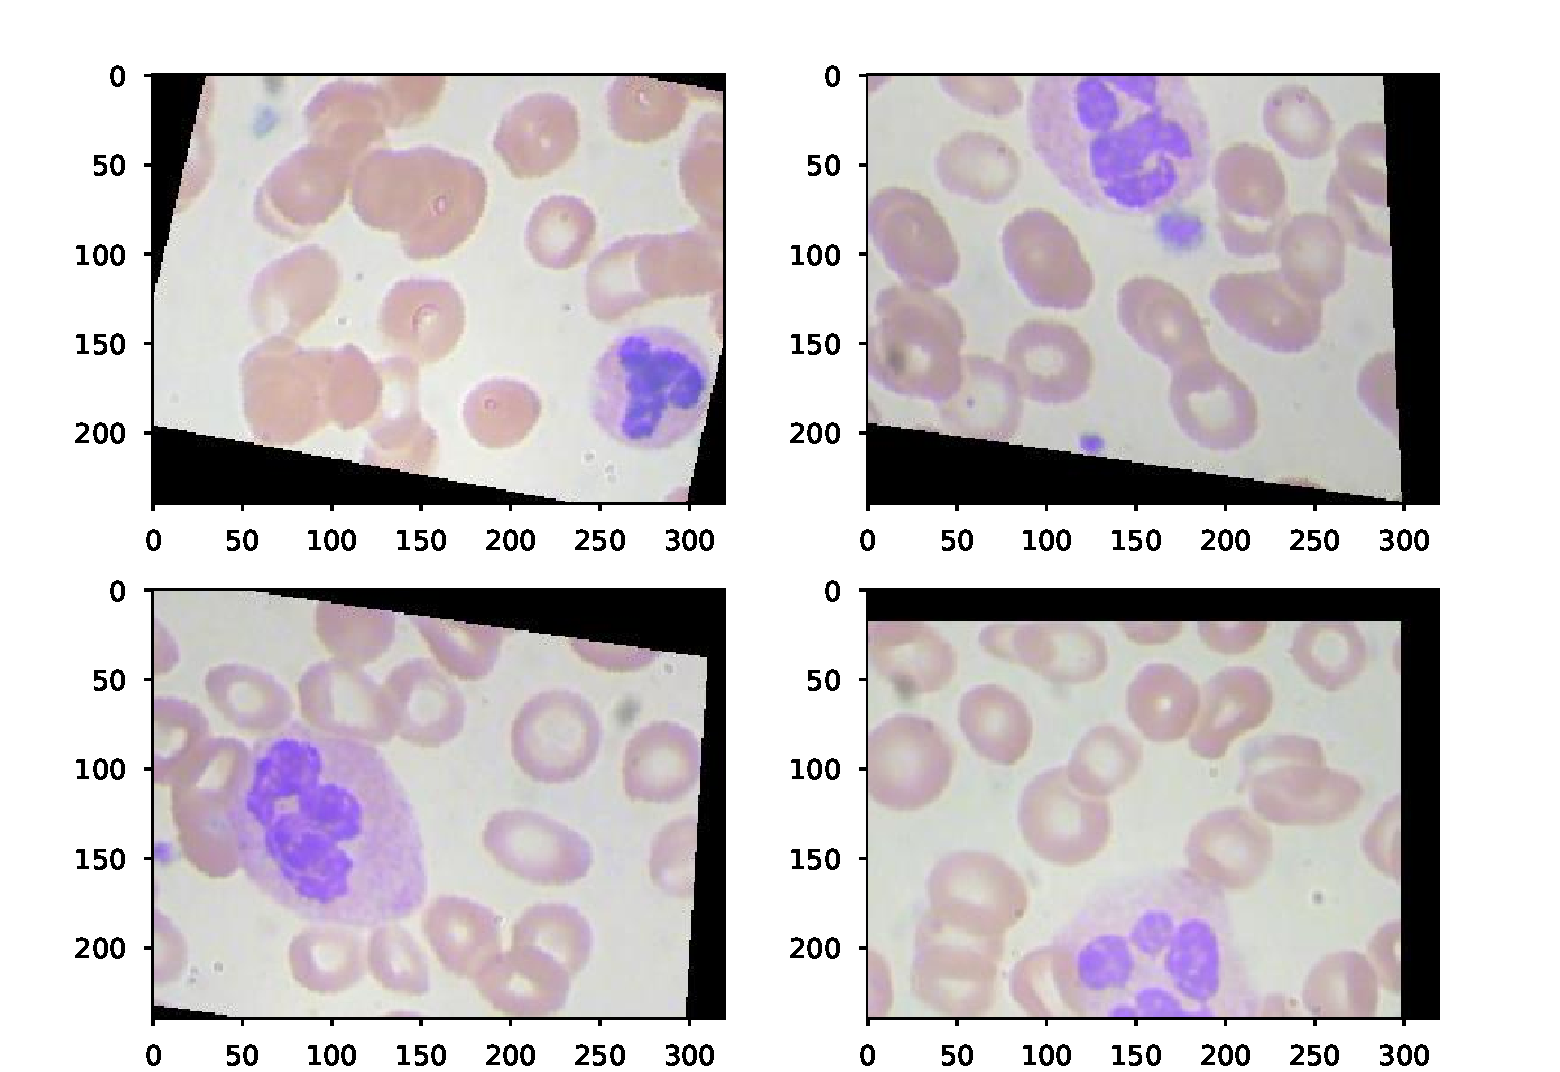
\includegraphics[width=0.5\textwidth]{Graphs/Neutrophils_originals.pdf}\label{fig:f1}}
  \hfill
  \subfloat[Lymphocytes]{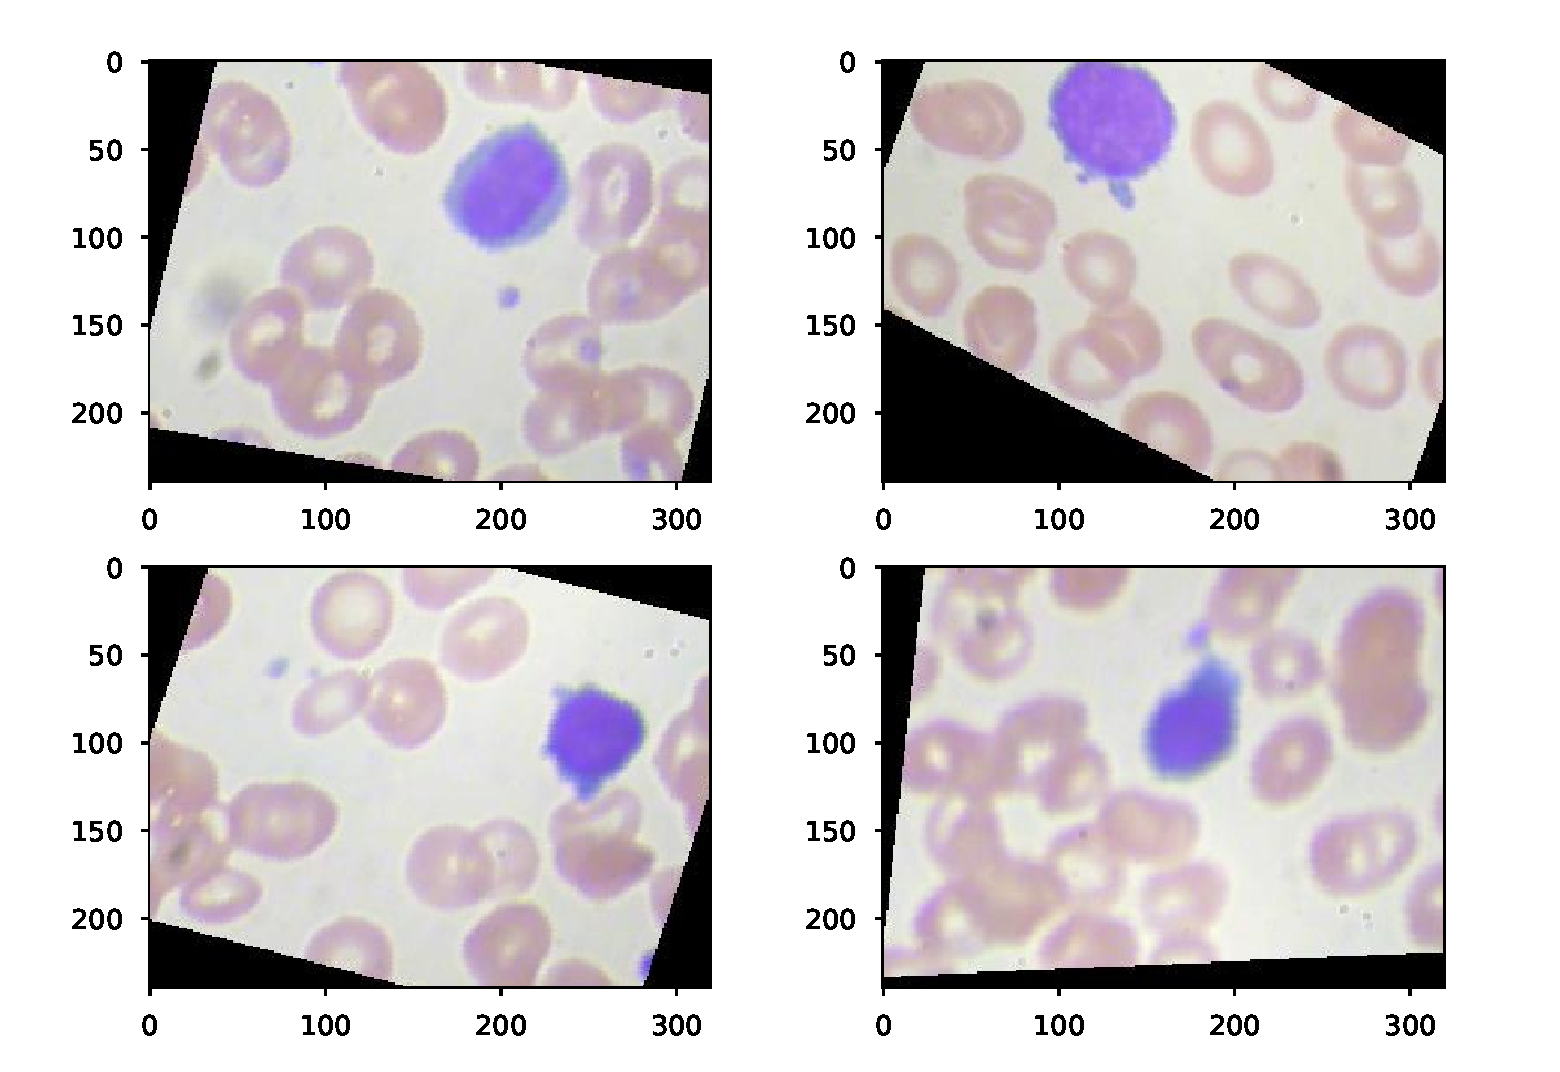
\includegraphics[width=0.5\textwidth]{Graphs/Lymphocytes_originals.pdf}\label{fig:f2}}
  \caption{Examples for both classes}\label{originals}
\end{figure}


\paragraph{}
The dataset consists in microscopic pictures of different kind of bloocells, it is available on Kaggle \cite{3}. There are four cells types in the dataset : Eosonophil, Lymphocyte, Monocyte, Neutrophil. We only concerned ourselves with a binary classification between Lymphocyte and Neutrophil. Since the images contain other cells in the background and since we are using a linear method, we made the choice of simplicity. To the human eye, the distinction between Lymphocytes and Neutrophils is the simplest to figure out since the former look "uni-nuclear" whereas the latter looks "poly-nuclear" (see \textbf{Figure \ref{originals}}). As a consequence, we thought this configuration would be the most likely to work.

\paragraph{}
We have indeed a problem regarding the focus of the images (see \textbf{Figure \ref{originals}}), since the cell of interest (the purple one) is never located at the same place within the images so we have to do a little pre-processing. We thus designed a procedure to crop the images around the centre of the cell of interest. In order to do so, we used the image processing library \textbf{opencv}. Our procedure to find the center of the cell is the following (more details can be found in our image processing notebook): 
\begin{enumerate}
	\item Blur the original image to make the contours of the cell of interest clearer and neutralize the contours of the other cells in the background.
	\item Convert the blurred image to grayscale.
	\item Neutralize the black pixels generated by framing issues by giving them the value of the average pixel of the rest of the image.
	\item Apply thresholding so that everything becomes white except the nucleus of the cell of interest.
	\item Apply negative morphology operation to remove the remaining "pepper noise".
	\item Find the center of cell by averaging the coordinates of the non white pixels and crop images around that center.
\end{enumerate}

The previous procedure applied to an example can be seen in \textbf{Figure  \ref{find_centre}} in the appendix. Examples of automatically cropped images can be seen in \textbf{Figure \ref{cropped}} in the appendix. We take the negative of the images so that the pixels of interest (the nucleus) are white and thus have the higher numerical values. From now on we used the transformed dataset containaing the cropped version of all the images, in grayscale and in negative.



\subsection {SDCA vs Pegasos on raw cropped images}

We flatten the images in order to work on vectors instead of matrices. Our cropped images are $120 \times 120$ pixels thus we are working with vectors in $\mathbb{R}^{120\times120} = \mathbb{R}^{14400}$. We have only $n=4982$ distributed approximately evenly between our two classes.


\paragraph{}
Since the two algorithm are stochastic, in order to perform a fair comparison we ran them each 100 times and then we averaged the evolution of losses, the CPU performances and the test scores. In term of CPU execution time, we timed only the updates for each epoch (meaning that all the extra computations coming from tracking losses, tracking score on test set etc... do not count in the CPU timer). We ran SDCA both with and without the modified-SGD first epoch. The results can be seen in \textbf{Figure \ref{comparison_original}}.


\begin{figure}[!tbp]
  \centering
  \subfloat[Loss (log scale) as a function of CPU time on train set]{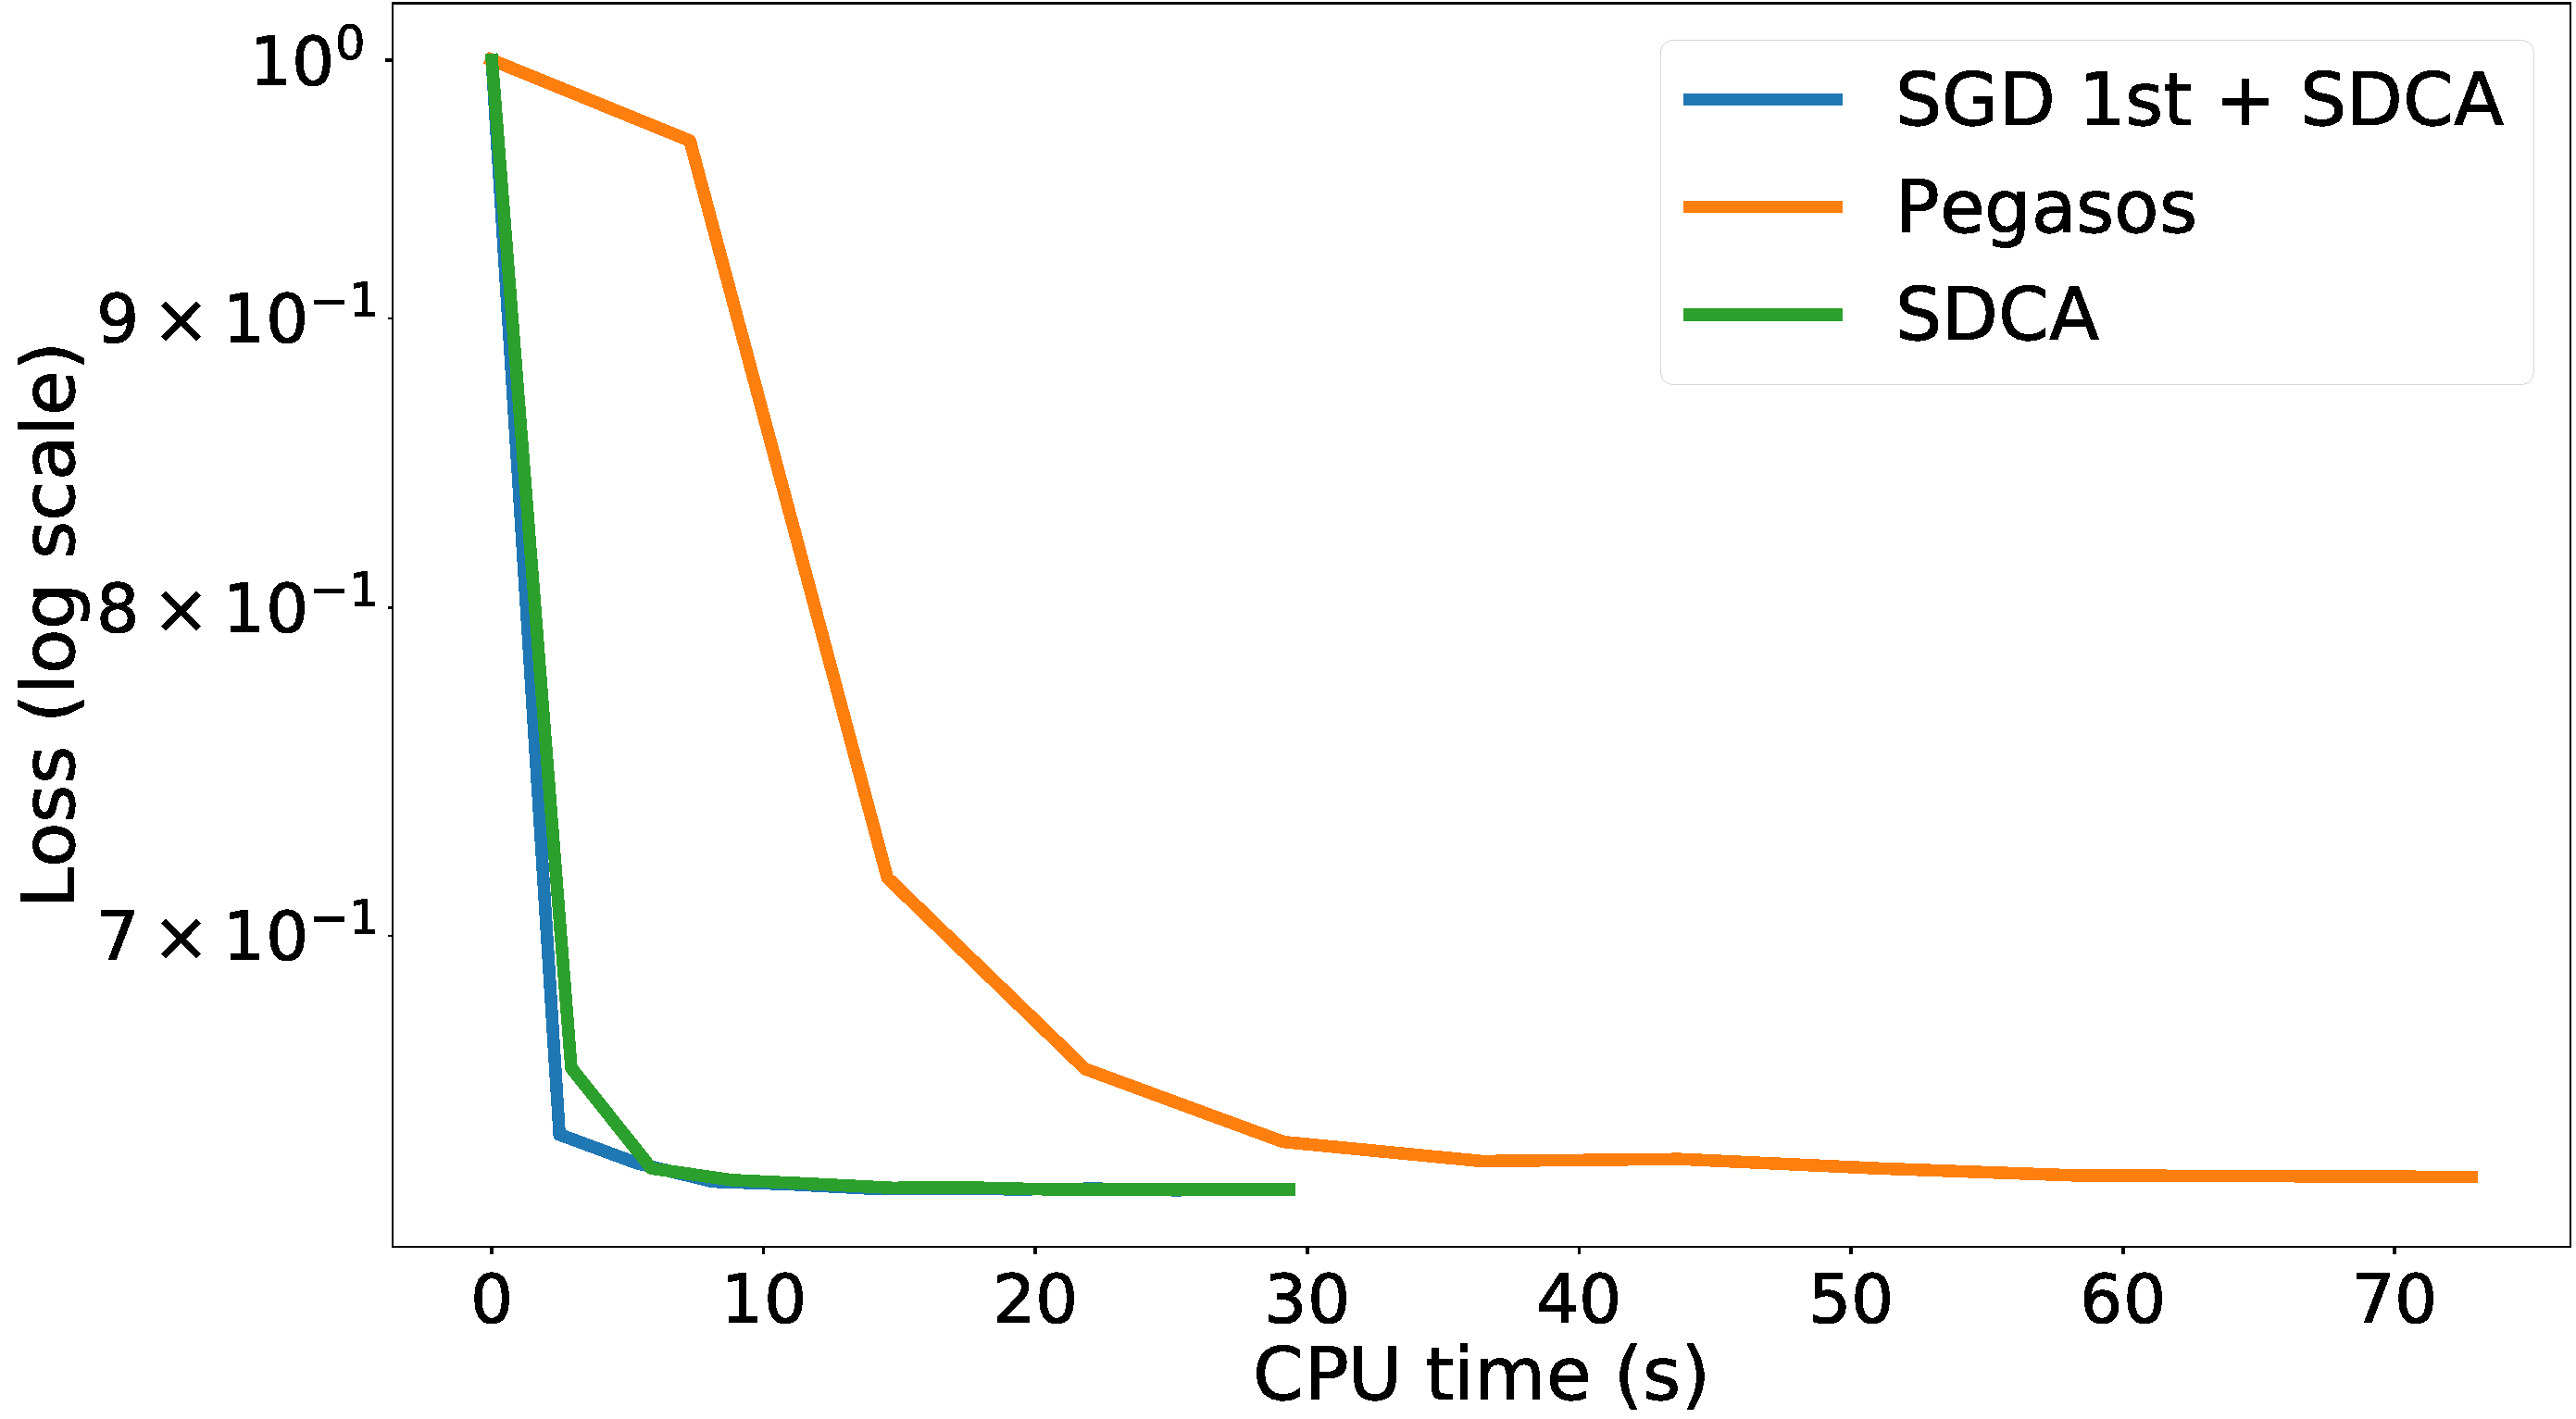
\includegraphics[width=0.5\textwidth]{Graphs/logloss_cpu_original3_mc100.pdf}}
  \hfill
  \subfloat[Error rate on test set as a function of number of epochs]{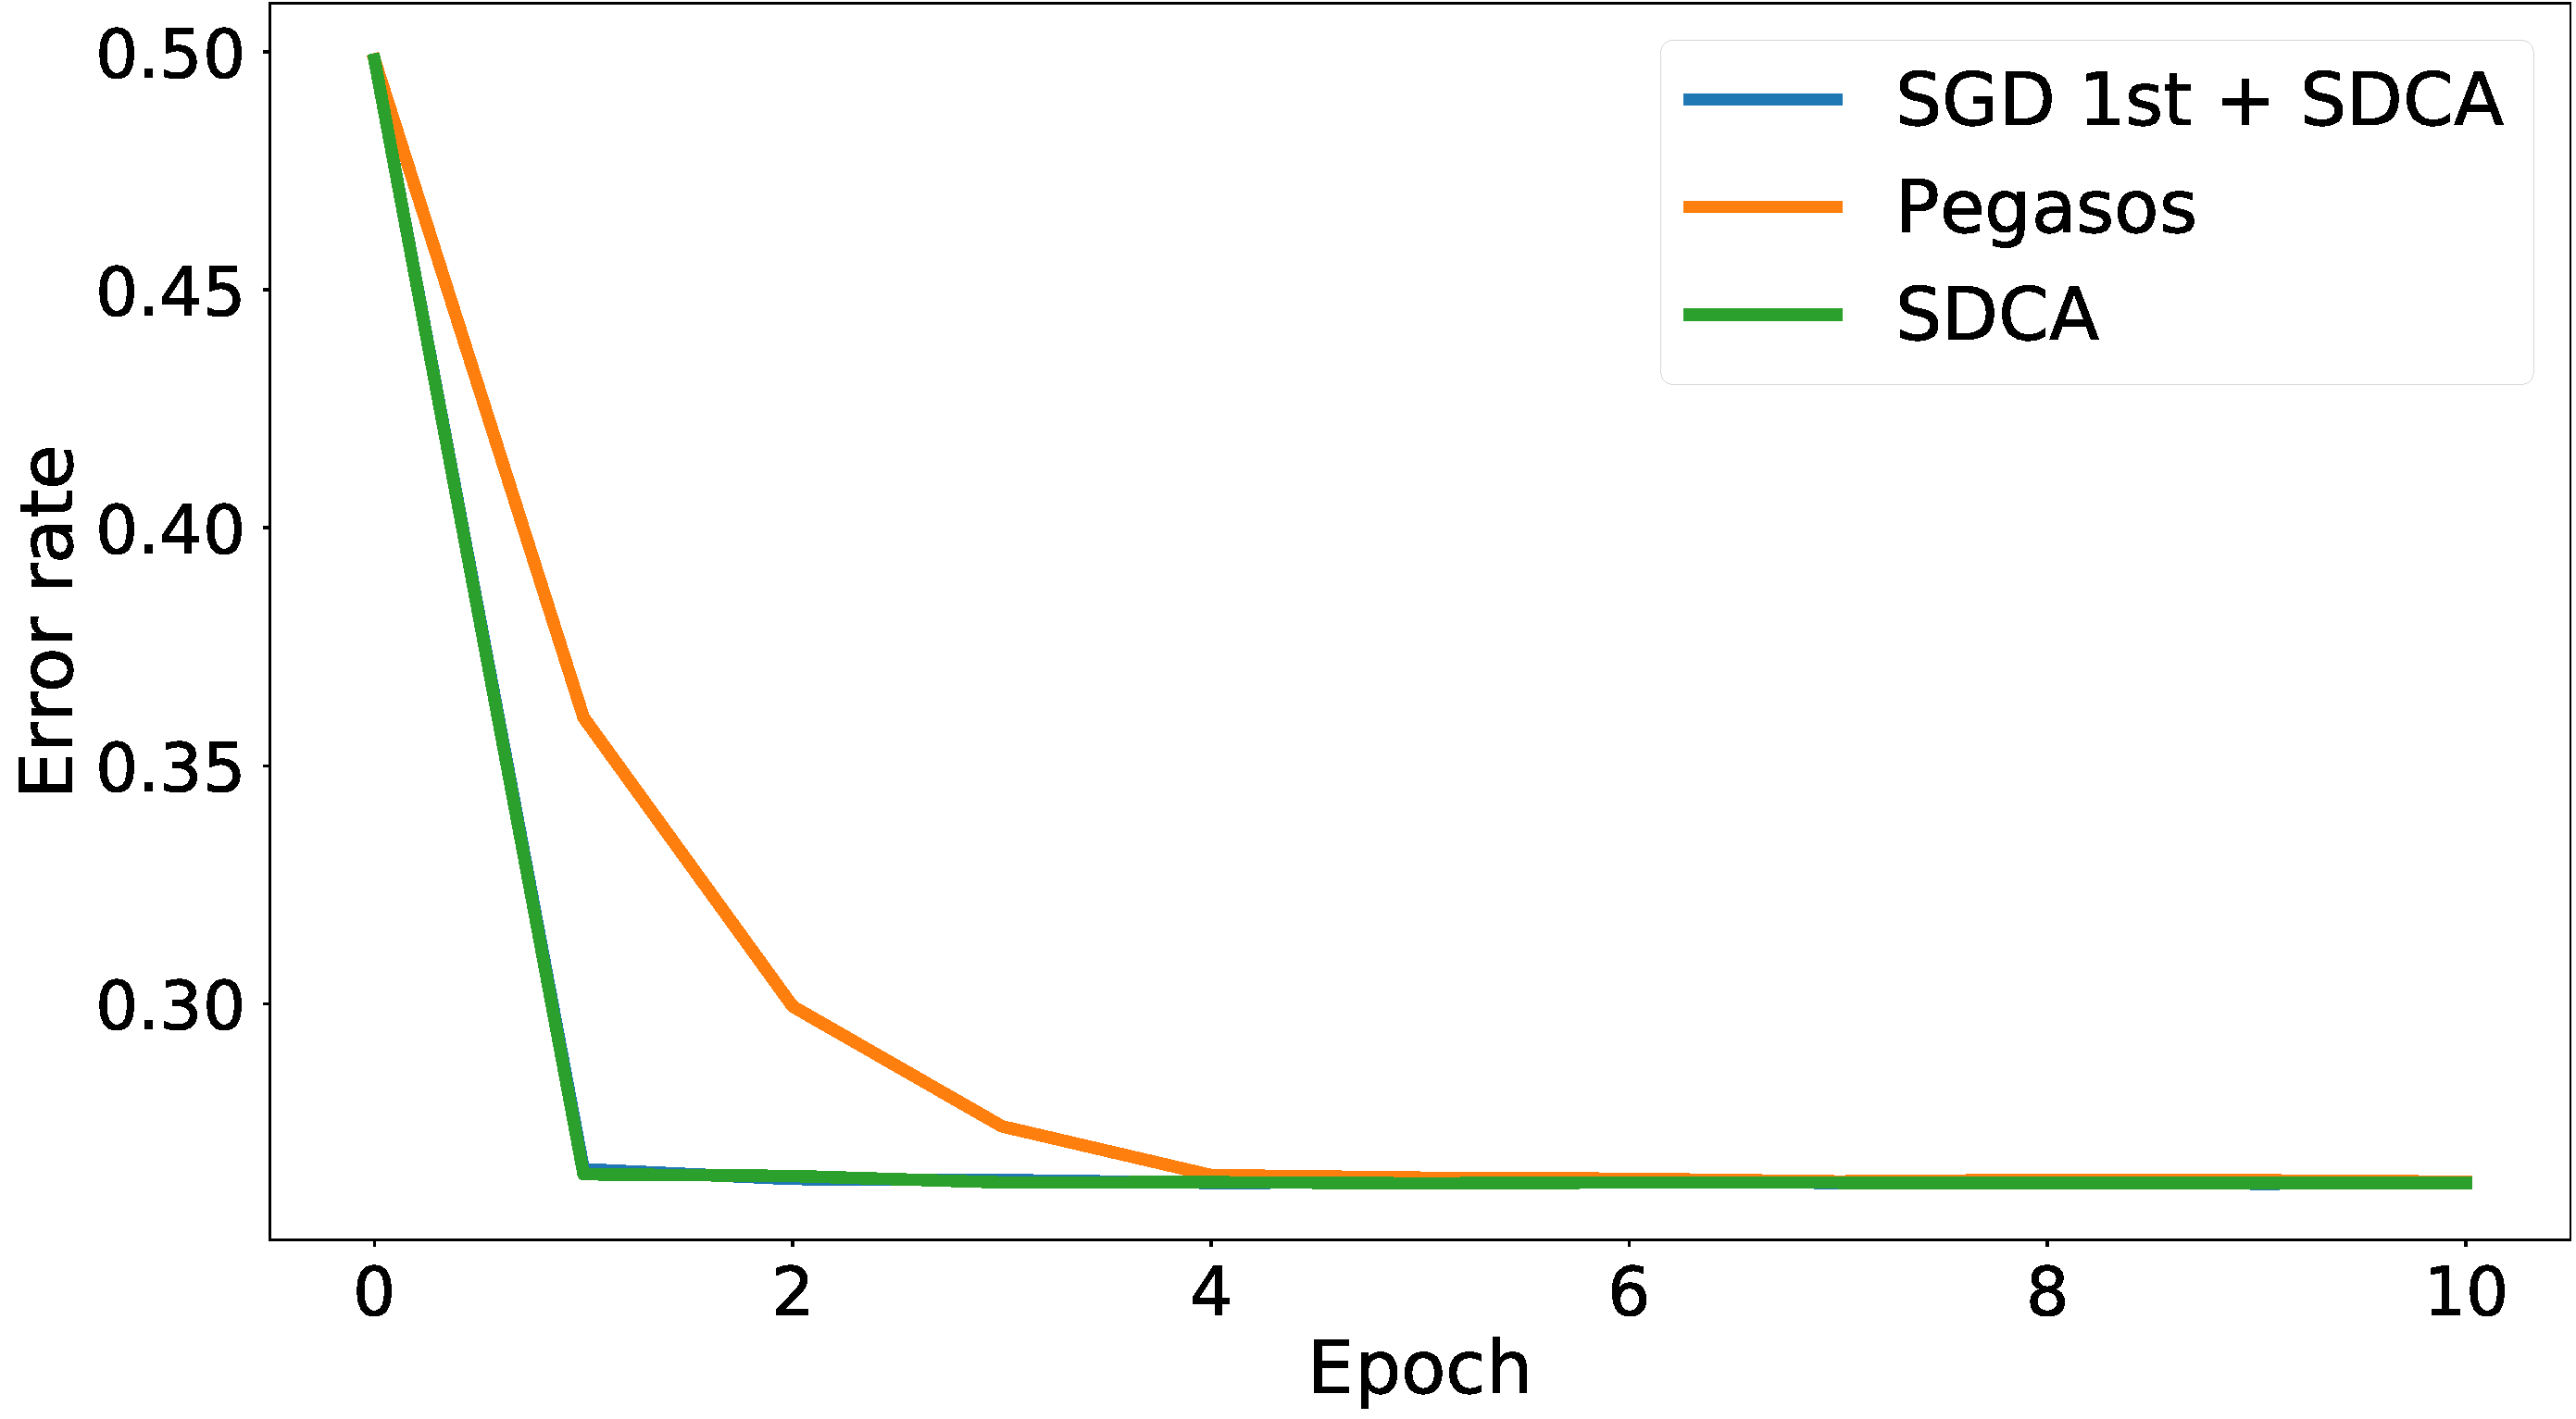
\includegraphics[width=0.5\textwidth]{Graphs/error_epoch_original3_mc100.pdf}}
  \hfill
  %\subfloat[Duality gap for SDCA as a function of number of epochs]{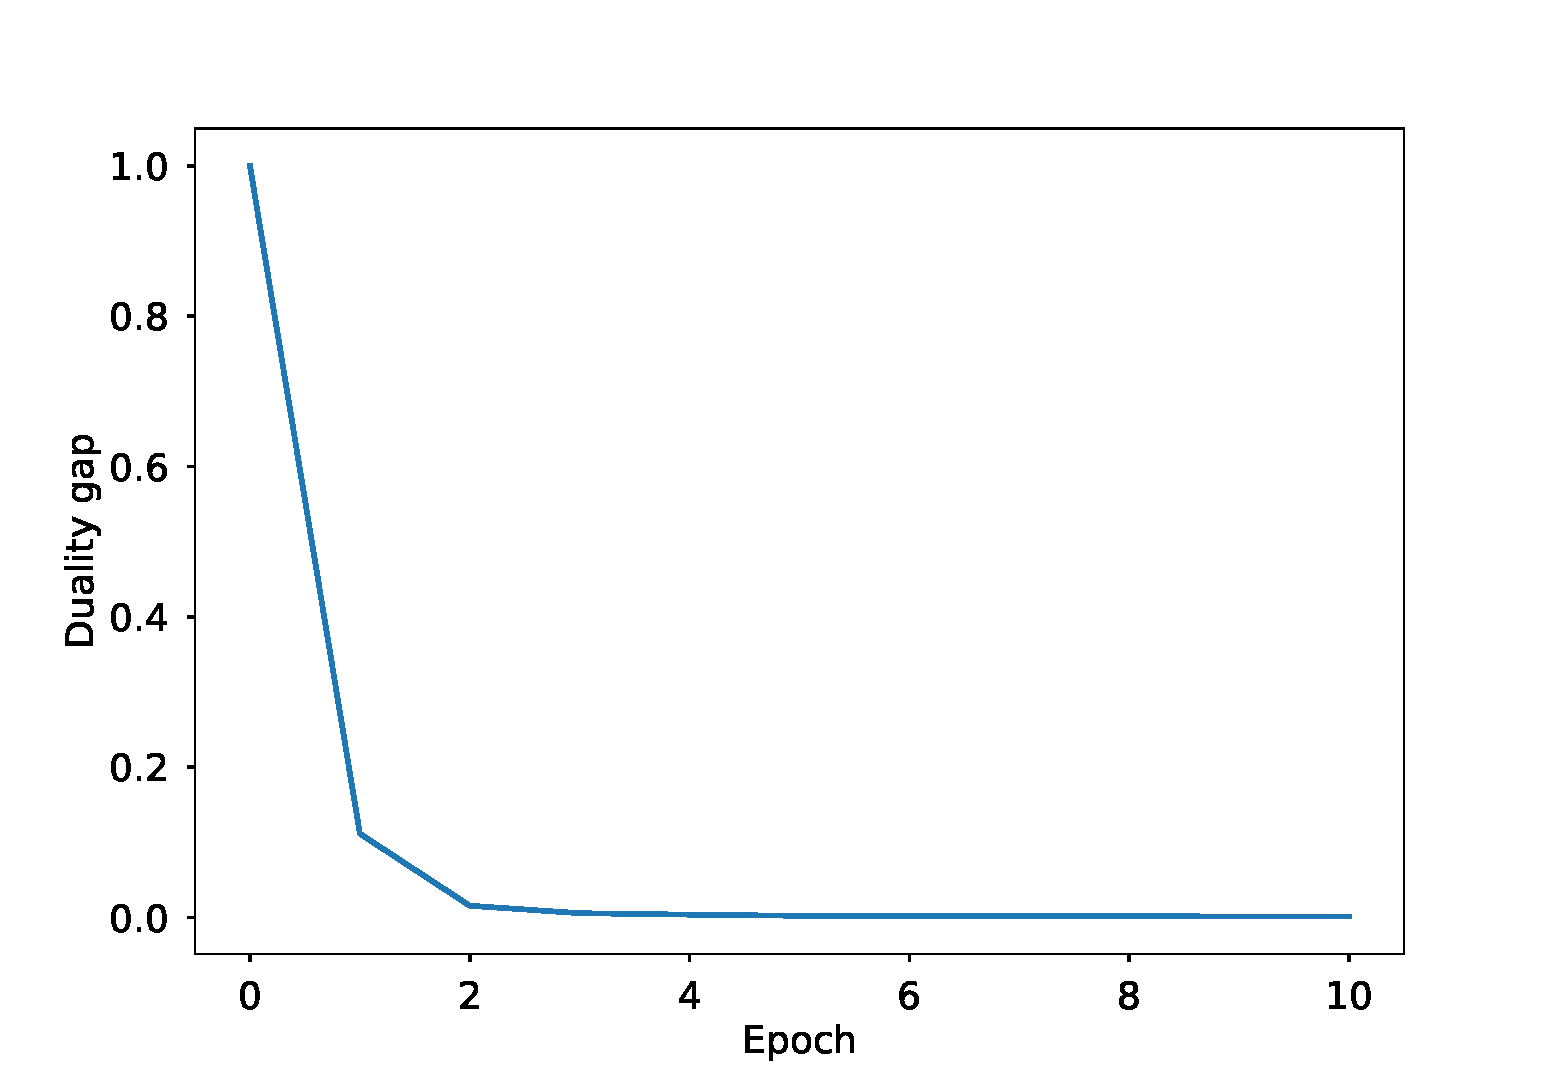
\includegraphics[width=0.5\textwidth]{Graphs/duality_original_mc100.pdf}}
  \caption{SDCA vs Pegasos - cropped vectorized images - averaged over 100 runs of each - $\lambda = 1.6$}\label{comparison_original}
\end{figure}

\paragraph{}
\textit{Remark 1: we deliberately called our time measure "CPU time" and not just "time" because under Linux, the Python timer do not return the wall clock - as it does under Windows - but rather the CPU time consumed for the execution of the timed task only}.

\paragraph{}
\textit{Remark 2: we deliberately set the duality gap stopping criterion to $0$ to be sure that all algorithms run for the same number of epochs to avoid averaging over lists of different sizes. Although the decrease in the duality gaps are plotted in the appendix in }.

\paragraph{}
\textit{Remark 3: after a few tries we set $\lambda=1.6$, although we did not cross-validate this. The minibatch size for Pegasos is set to 100.}


\paragraph{}
Panel \textbf{(a)} of \textbf{Figure \ref{comparison_original}} represents the loss as a function of cumulated CPU time. We can see that SDCA (with and without SGD as first epoch) runs actually a lot faster than Pegasos, the latter taking $\approx$ 3 times longer to reach convergence than the former.  If we look at the panel \textbf{(b)} of the same figure, SDCA and SDCA with SGD reach the best score ($\approx$ 26 \%) after only 2 epochs, whereas Pegasos stabilizes itself around the 4-th epoch. 


\paragraph{}
To finish with, the modified-SGD epoch brings faster loss reduction in the first epoch but the improvement does not translate in terms of score on the test set where the two version of SDCA have exactly the same performances.

\paragraph{}
The data used for this comparison is very noisy (for one, there are lots of variations in the background of the images which carry no information whatsoever) and we have way more dimensions than data points ($d>>n$). This may result in poor subgradient estimations in Pegasos. For that matter it seems that SDCA is more robust than Pegasos, maybe it is what the authors of \cite{1} means by "more precise". We will now take the comparison to an easier context by performing dimensionnality reduction using principal component analysis (PCA).


\FloatBarrier
\subsection {SDCA vs Pegasos with PCA dimensionality reduction}

We now run the same algorithms but we proceed to a PCA decomposition of the training set matrix. Looking at the plot of the resulting first 1000 singular values (see \textbf{Figure \ref{pca_decrease}} in the appendix) and since we want to cut out the effect of the background "noise" we keep only the coordinate of the projection on the principal components associated with the $40$ greater singular values, thus now $d=40$ and $d << n$. The representation of some images associated with this projection can be seen in \textbf{Figure \ref{pca_reduced}} in the appendix. As in the previous subsection, we average over 100 runs of the algorithms.




\begin{figure}[!tbp]
  \centering
  \subfloat[Loss (log scale) as a function of CPU time on train set]{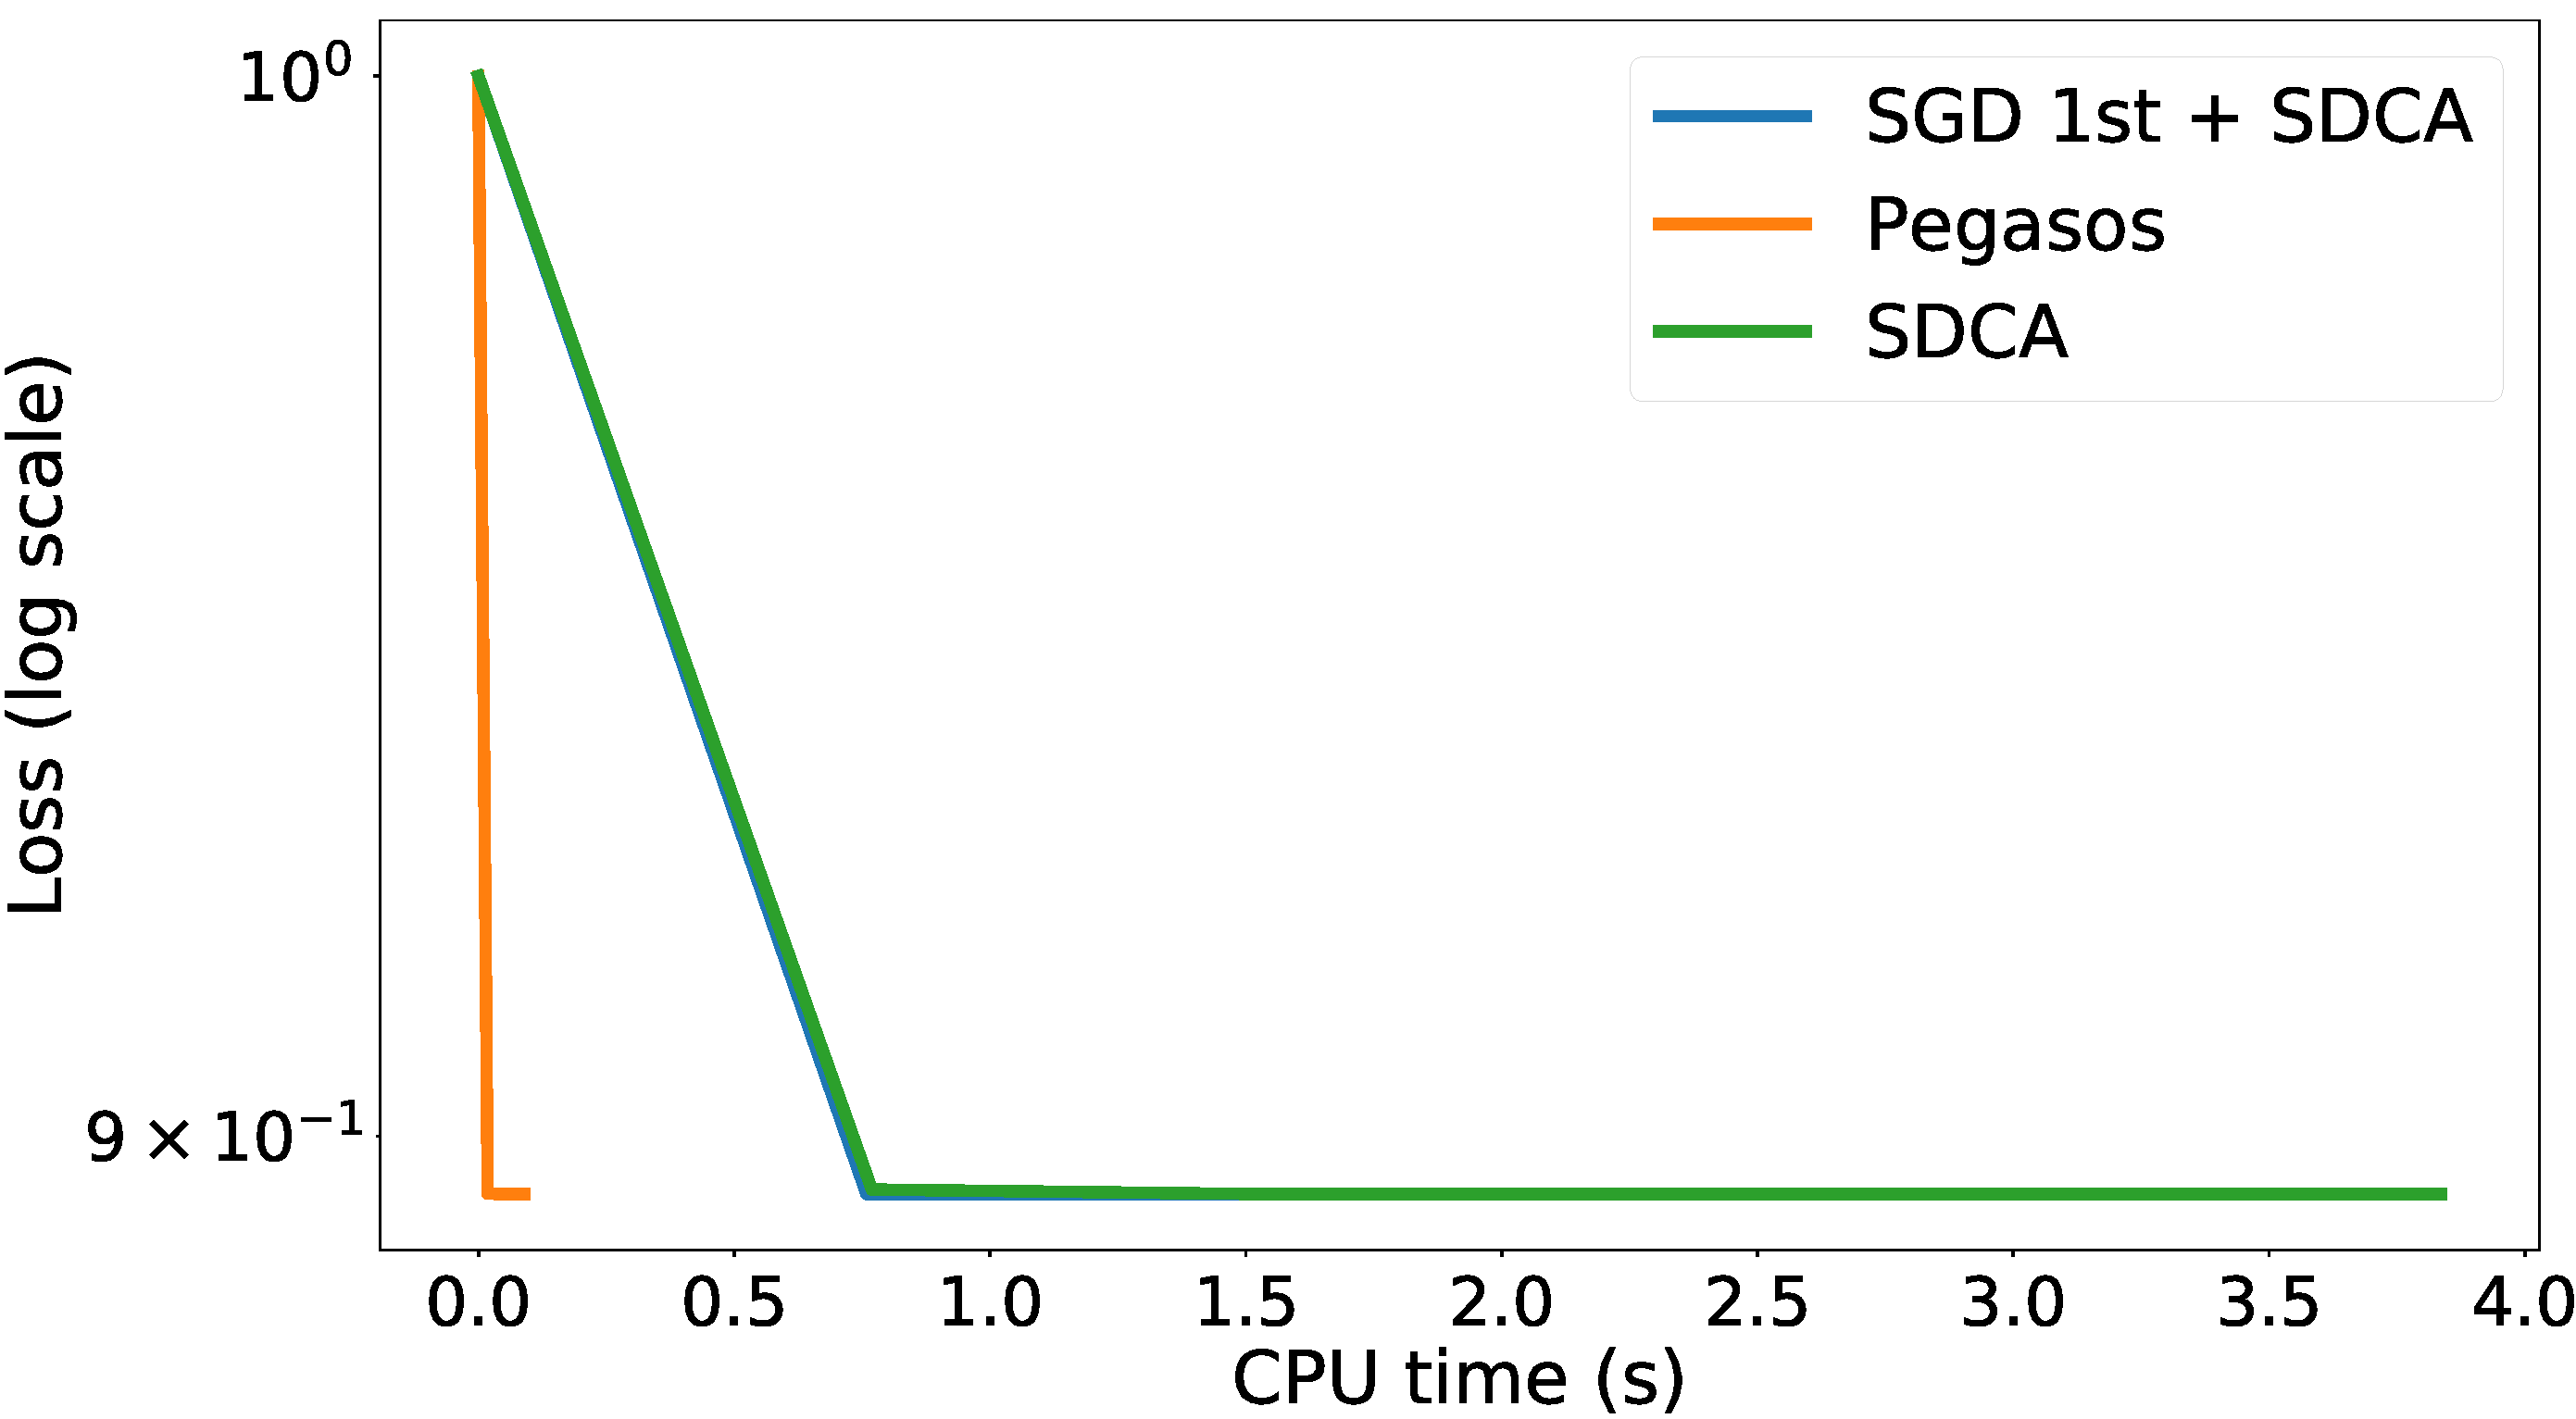
\includegraphics[width=0.5\textwidth]{Graphs/logloss_cpu_pca3_mc100.pdf}}
  \hfill
  \subfloat[Error rate on test set as a function of number of epochs]{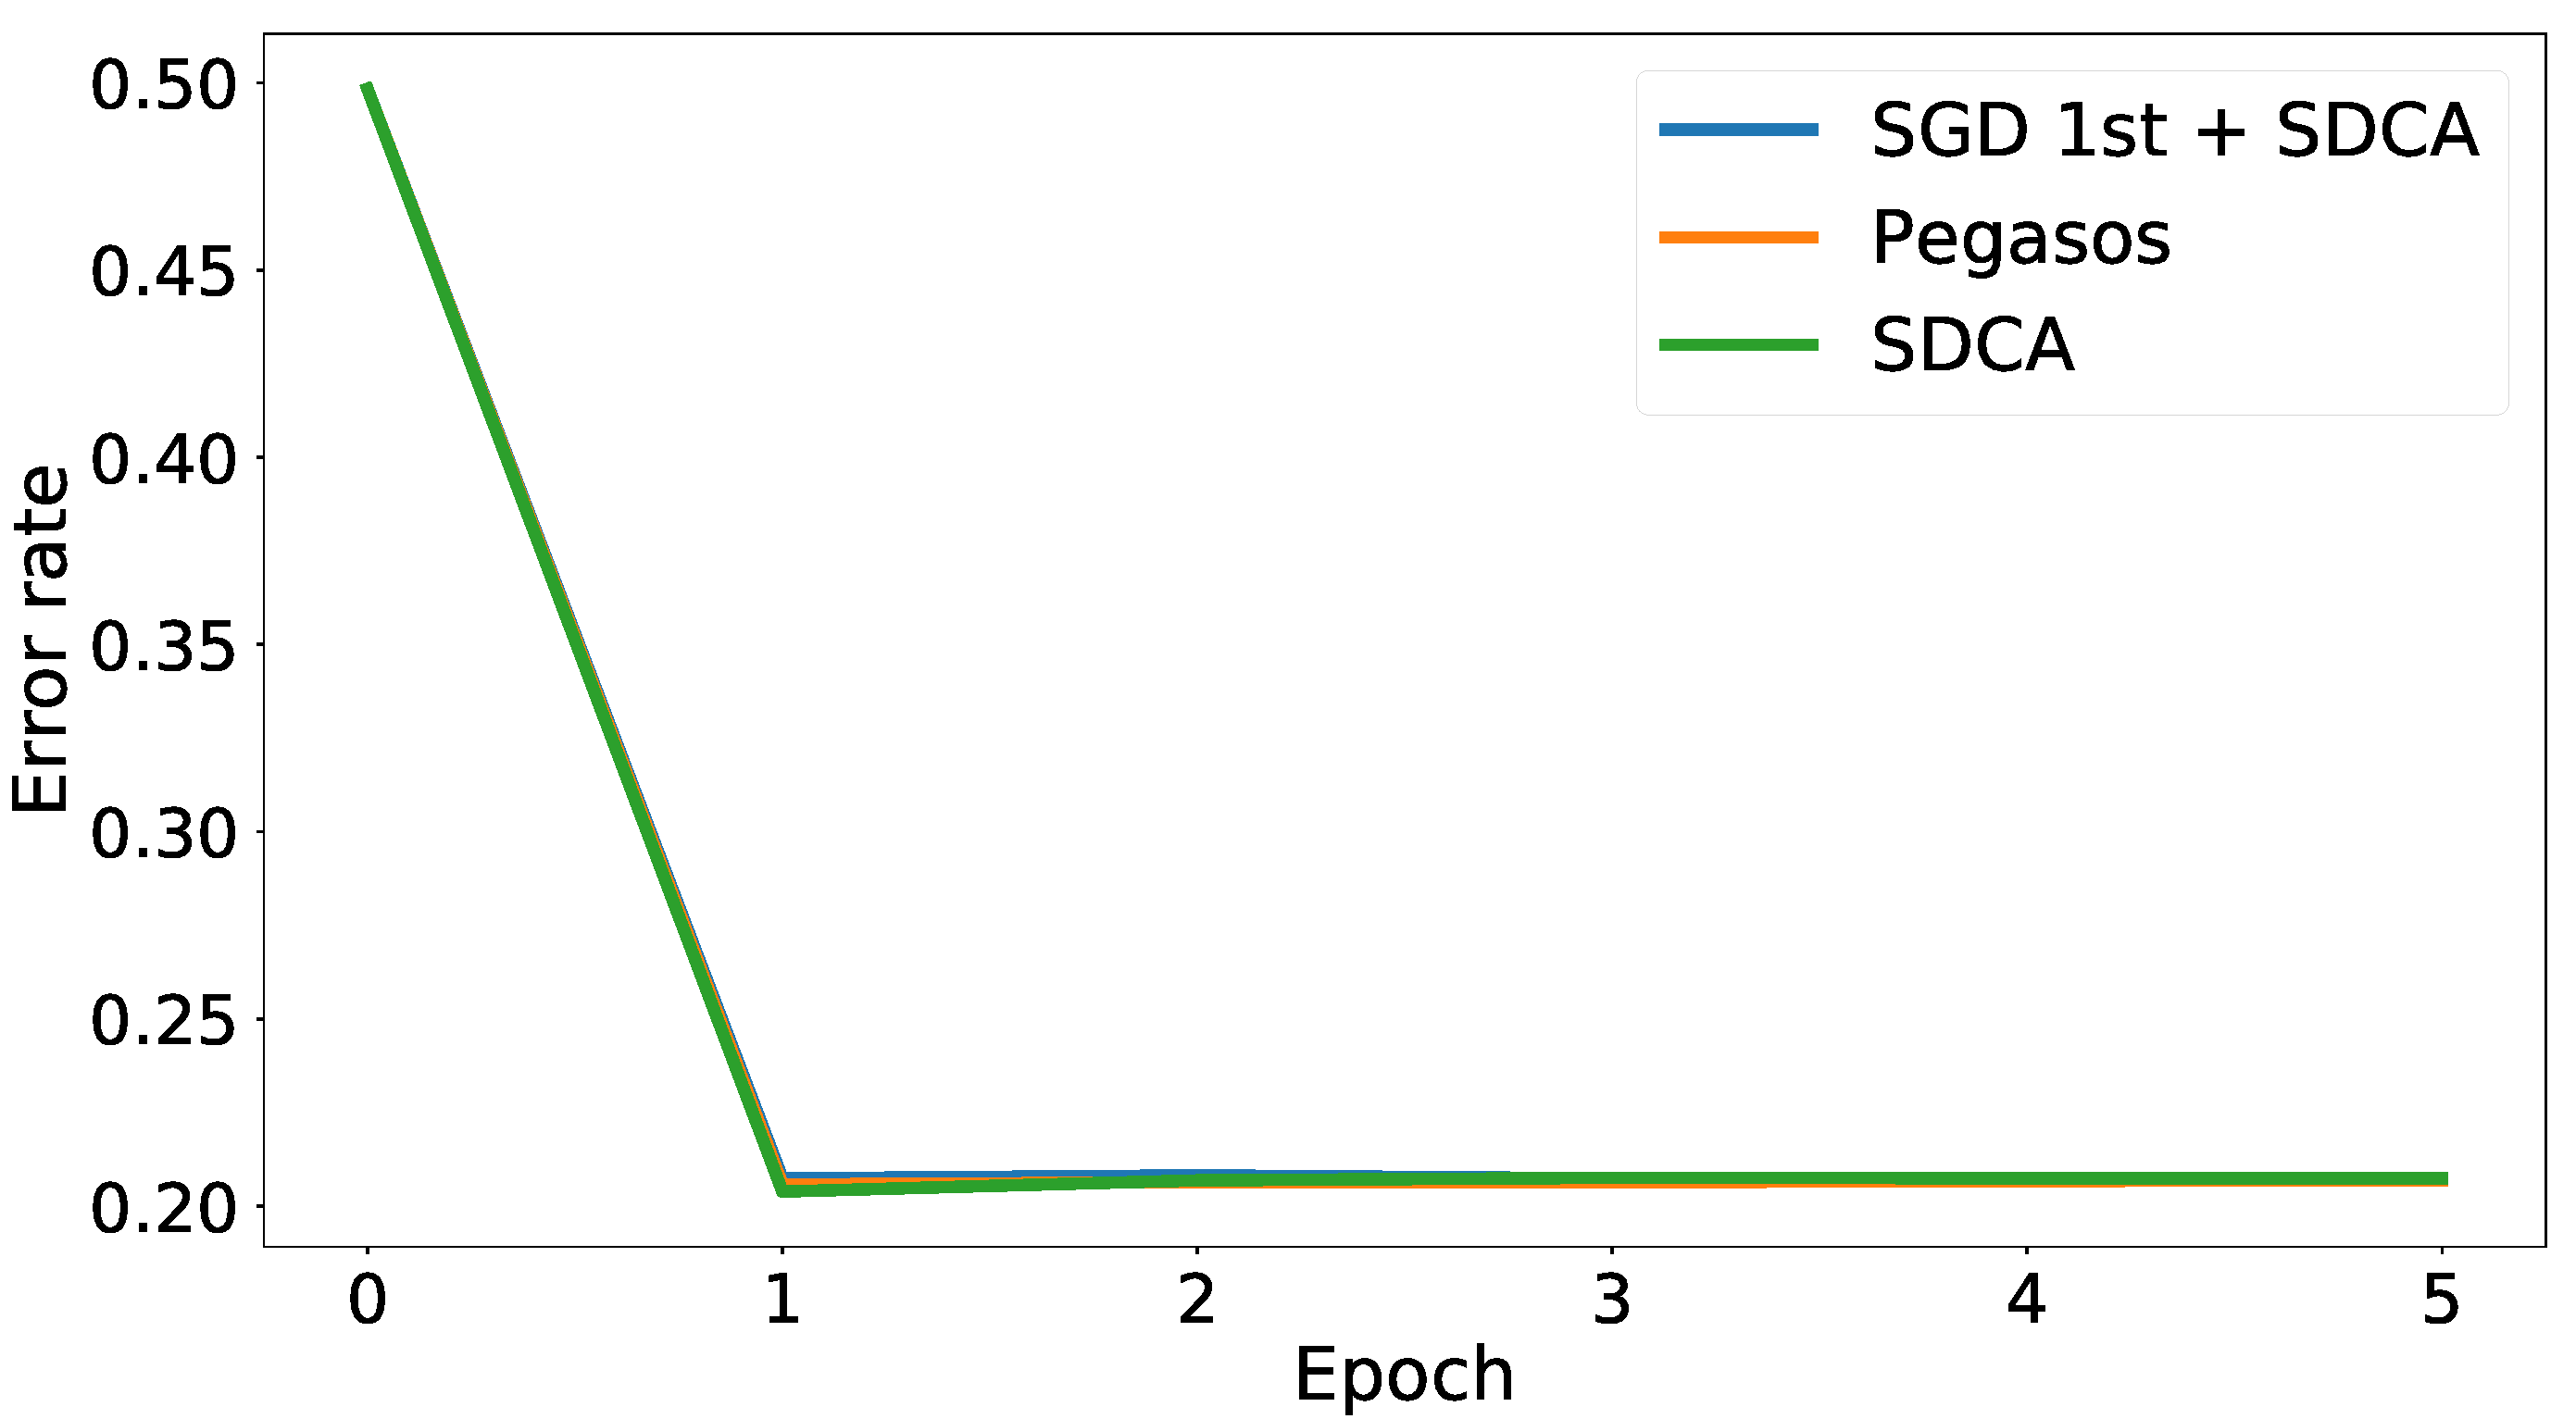
\includegraphics[width=0.5\textwidth]{Graphs/error_epoch_pca3_mc100.pdf}}
  \hfill
  %\subfloat[Duality gap for SDCA as a function of number of epochs]{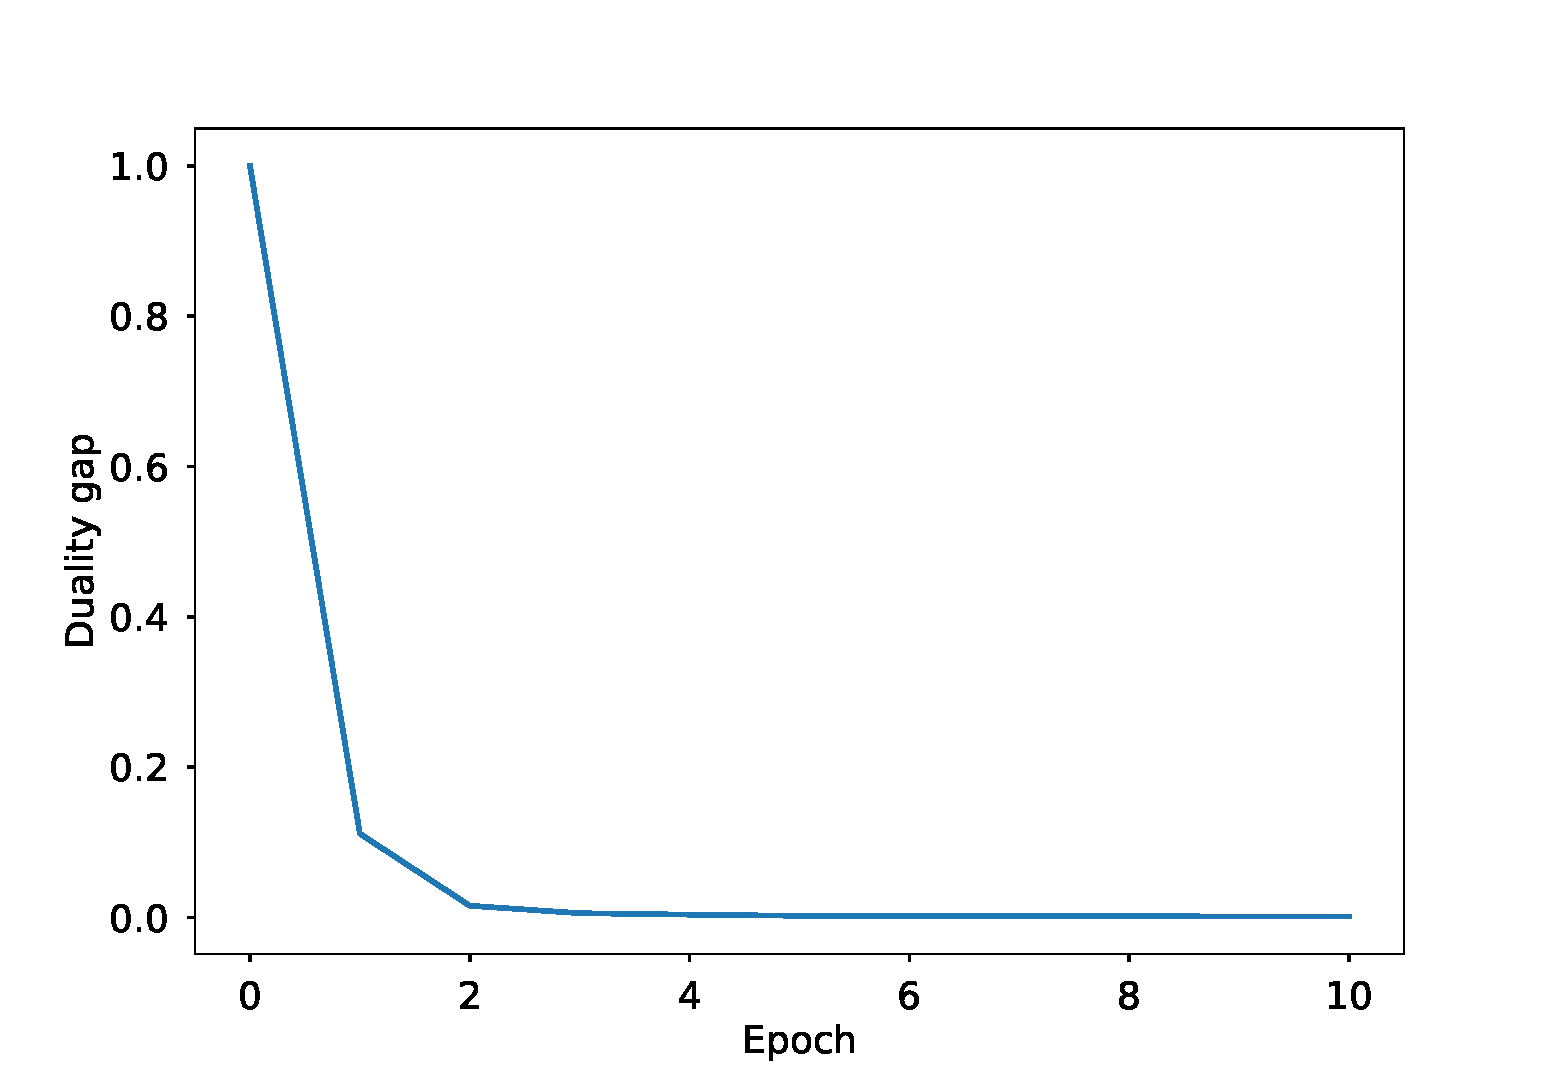
\includegraphics[width=0.5\textwidth]{Graphs/duality_original_mc100.pdf}}
  \caption{SDCA vs Pegasos - PCA reduced (40) - averaged over 100 runs - $\lambda = 1.6$}\label{comparison_pca}
\end{figure}


\paragraph{}
We can see in \textbf{Figure \ref{comparison_pca}} that, as opposed to the previous configuration (raw vectorized images), all three algorithms behaves the same in terms of score on test set (see panel \textbf{(b)}). We may explain this by the dimension reduction, which hopefully cuts out some background noise. This may help reduce the variance in the estimation of the gradient for Pegasos.

\paragraph{}
Also, panels \textbf{(a)} shows us that in this configuration, Pegasos runs its epochs way faster than both versions of SDCA. It probably because Pegasos is a primal algorithm so it performs its computations and updates in $\mathbb{R}^d$ whereas SDCA is a primal-dual algorithm so it performs both dual updates in $\mathbb{R}^n$ and primal updates in $\mathbb{R}^d$. Now that $d (=40) << n(\approx 5000)$, this is only logical to see Pegasos run faster. 

%This is probably a mechanical effect of the dimension reduction. Pegasos is a primal algorithm so the number of computations and coordinate modifications per update scales in $d$ whereas SDCA performs both primal (in $d$) and dual updates 

\section{Conclusions}



\printbibliography

\newpage

\appendix

\FloatBarrier
\section{Automatic cropping procedure}

\begin{figure}[!htb]
  \centering
  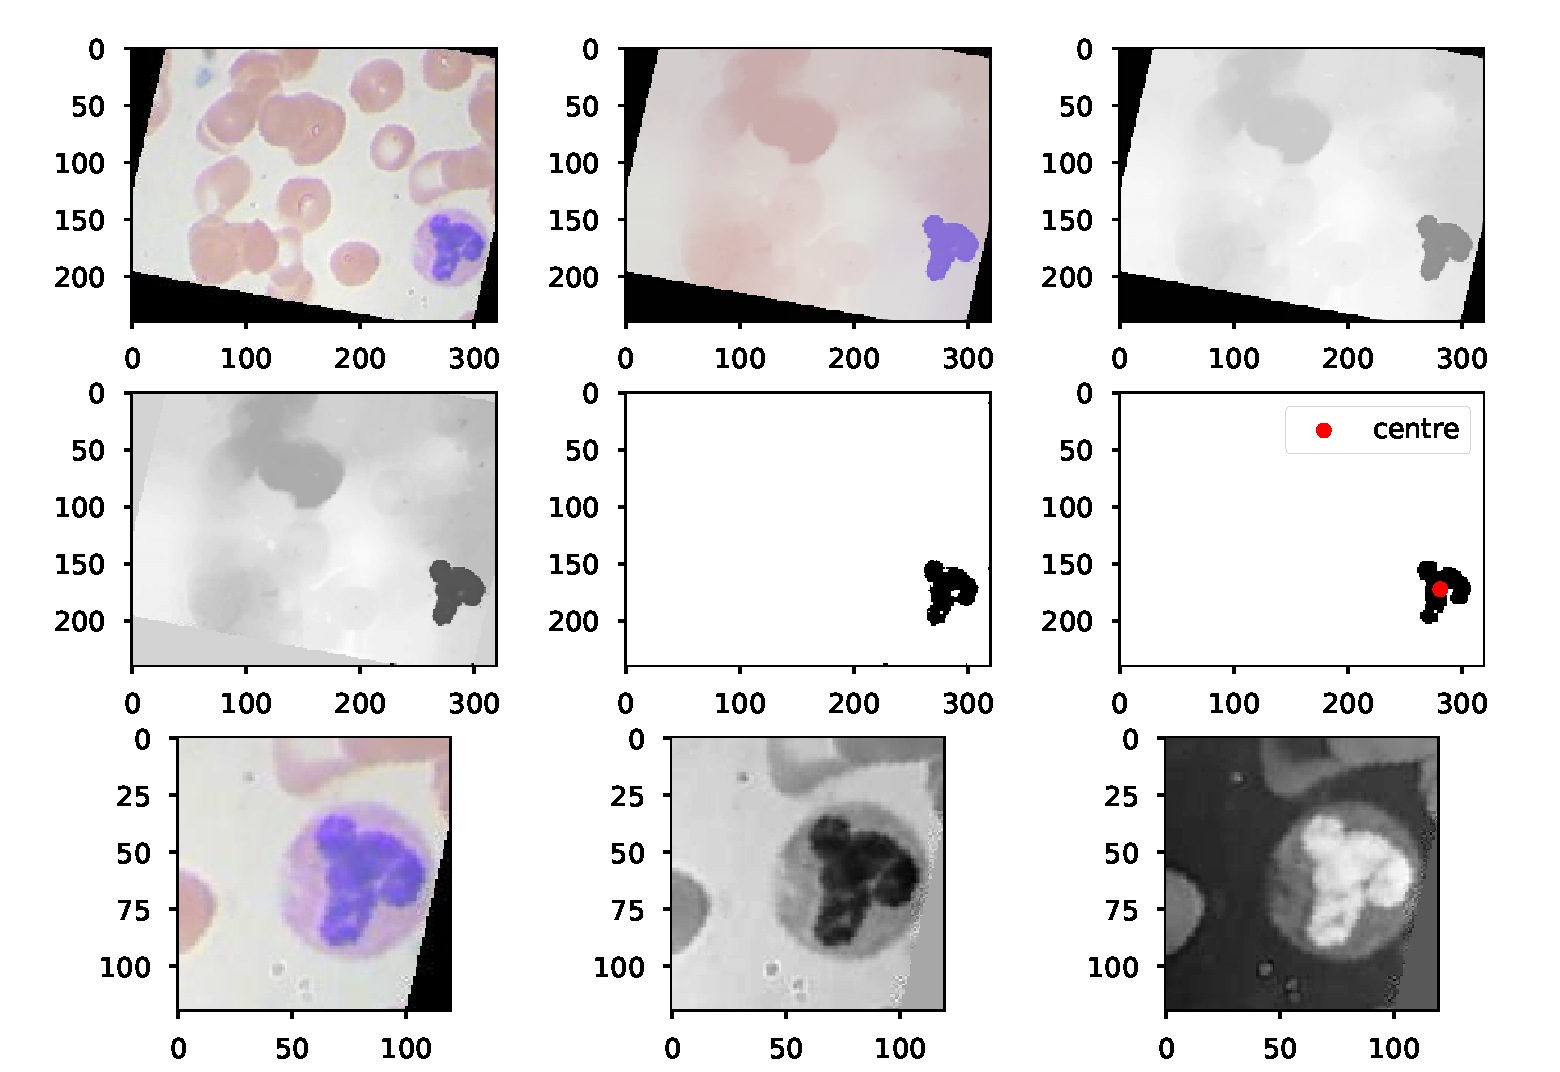
\includegraphics[width=0.85\textwidth]{Graphs/Find_center.pdf}
  \caption{Automatic cropping procedure}\label{find_centre}
\end{figure}


\begin{figure}[!htb]
  \centering
  \subfloat[Cropped neutrophils]{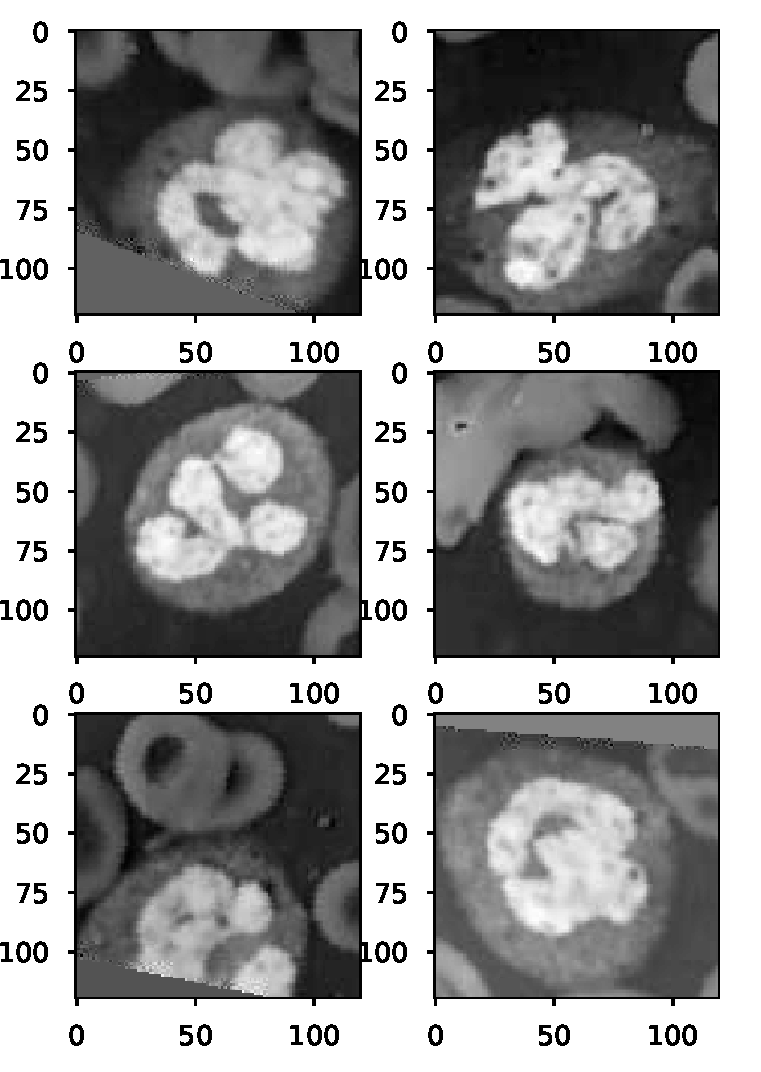
\includegraphics[width=0.4\textwidth]{Graphs/cropped_neutro.pdf}}
  \hfill
  \subfloat[Cropped lymphocytes]{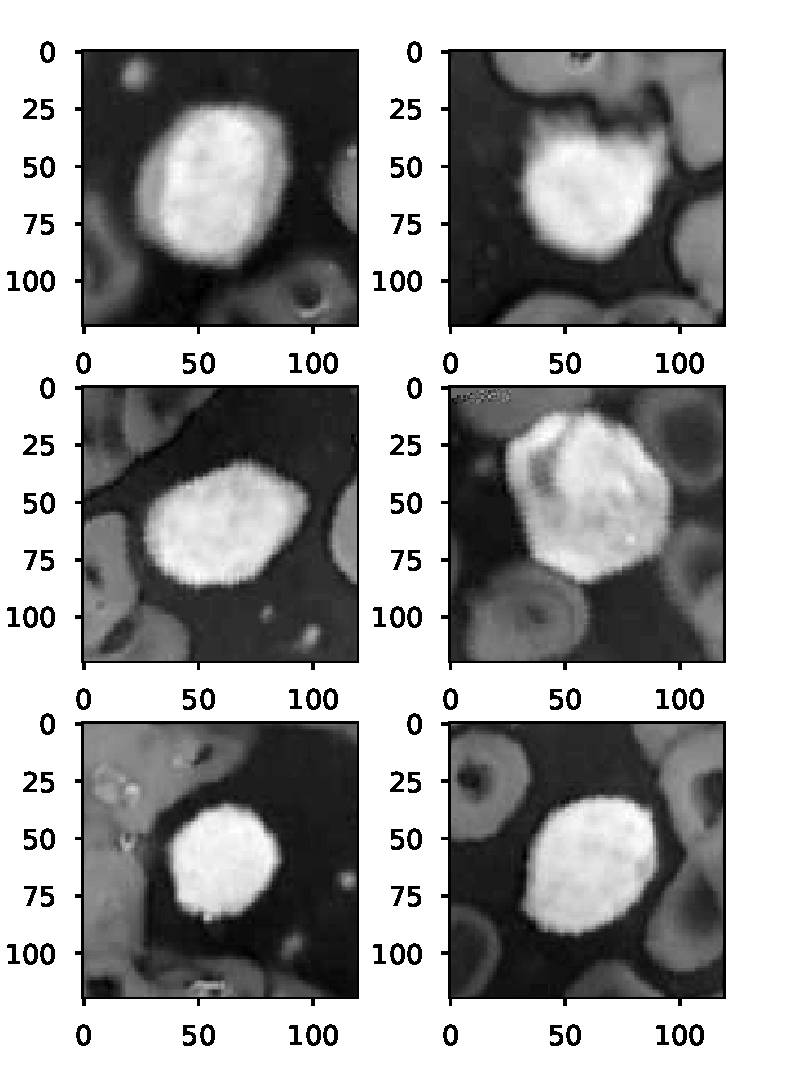
\includegraphics[width=0.42\textwidth]{Graphs/cropped_lymph.pdf}}
  \caption{Automatically cropped images for both classes}\label{cropped}
\end{figure}

\newpage

\FloatBarrier

\section{SDCA duality gaps}

\begin{figure}[!htb]
	\centering
	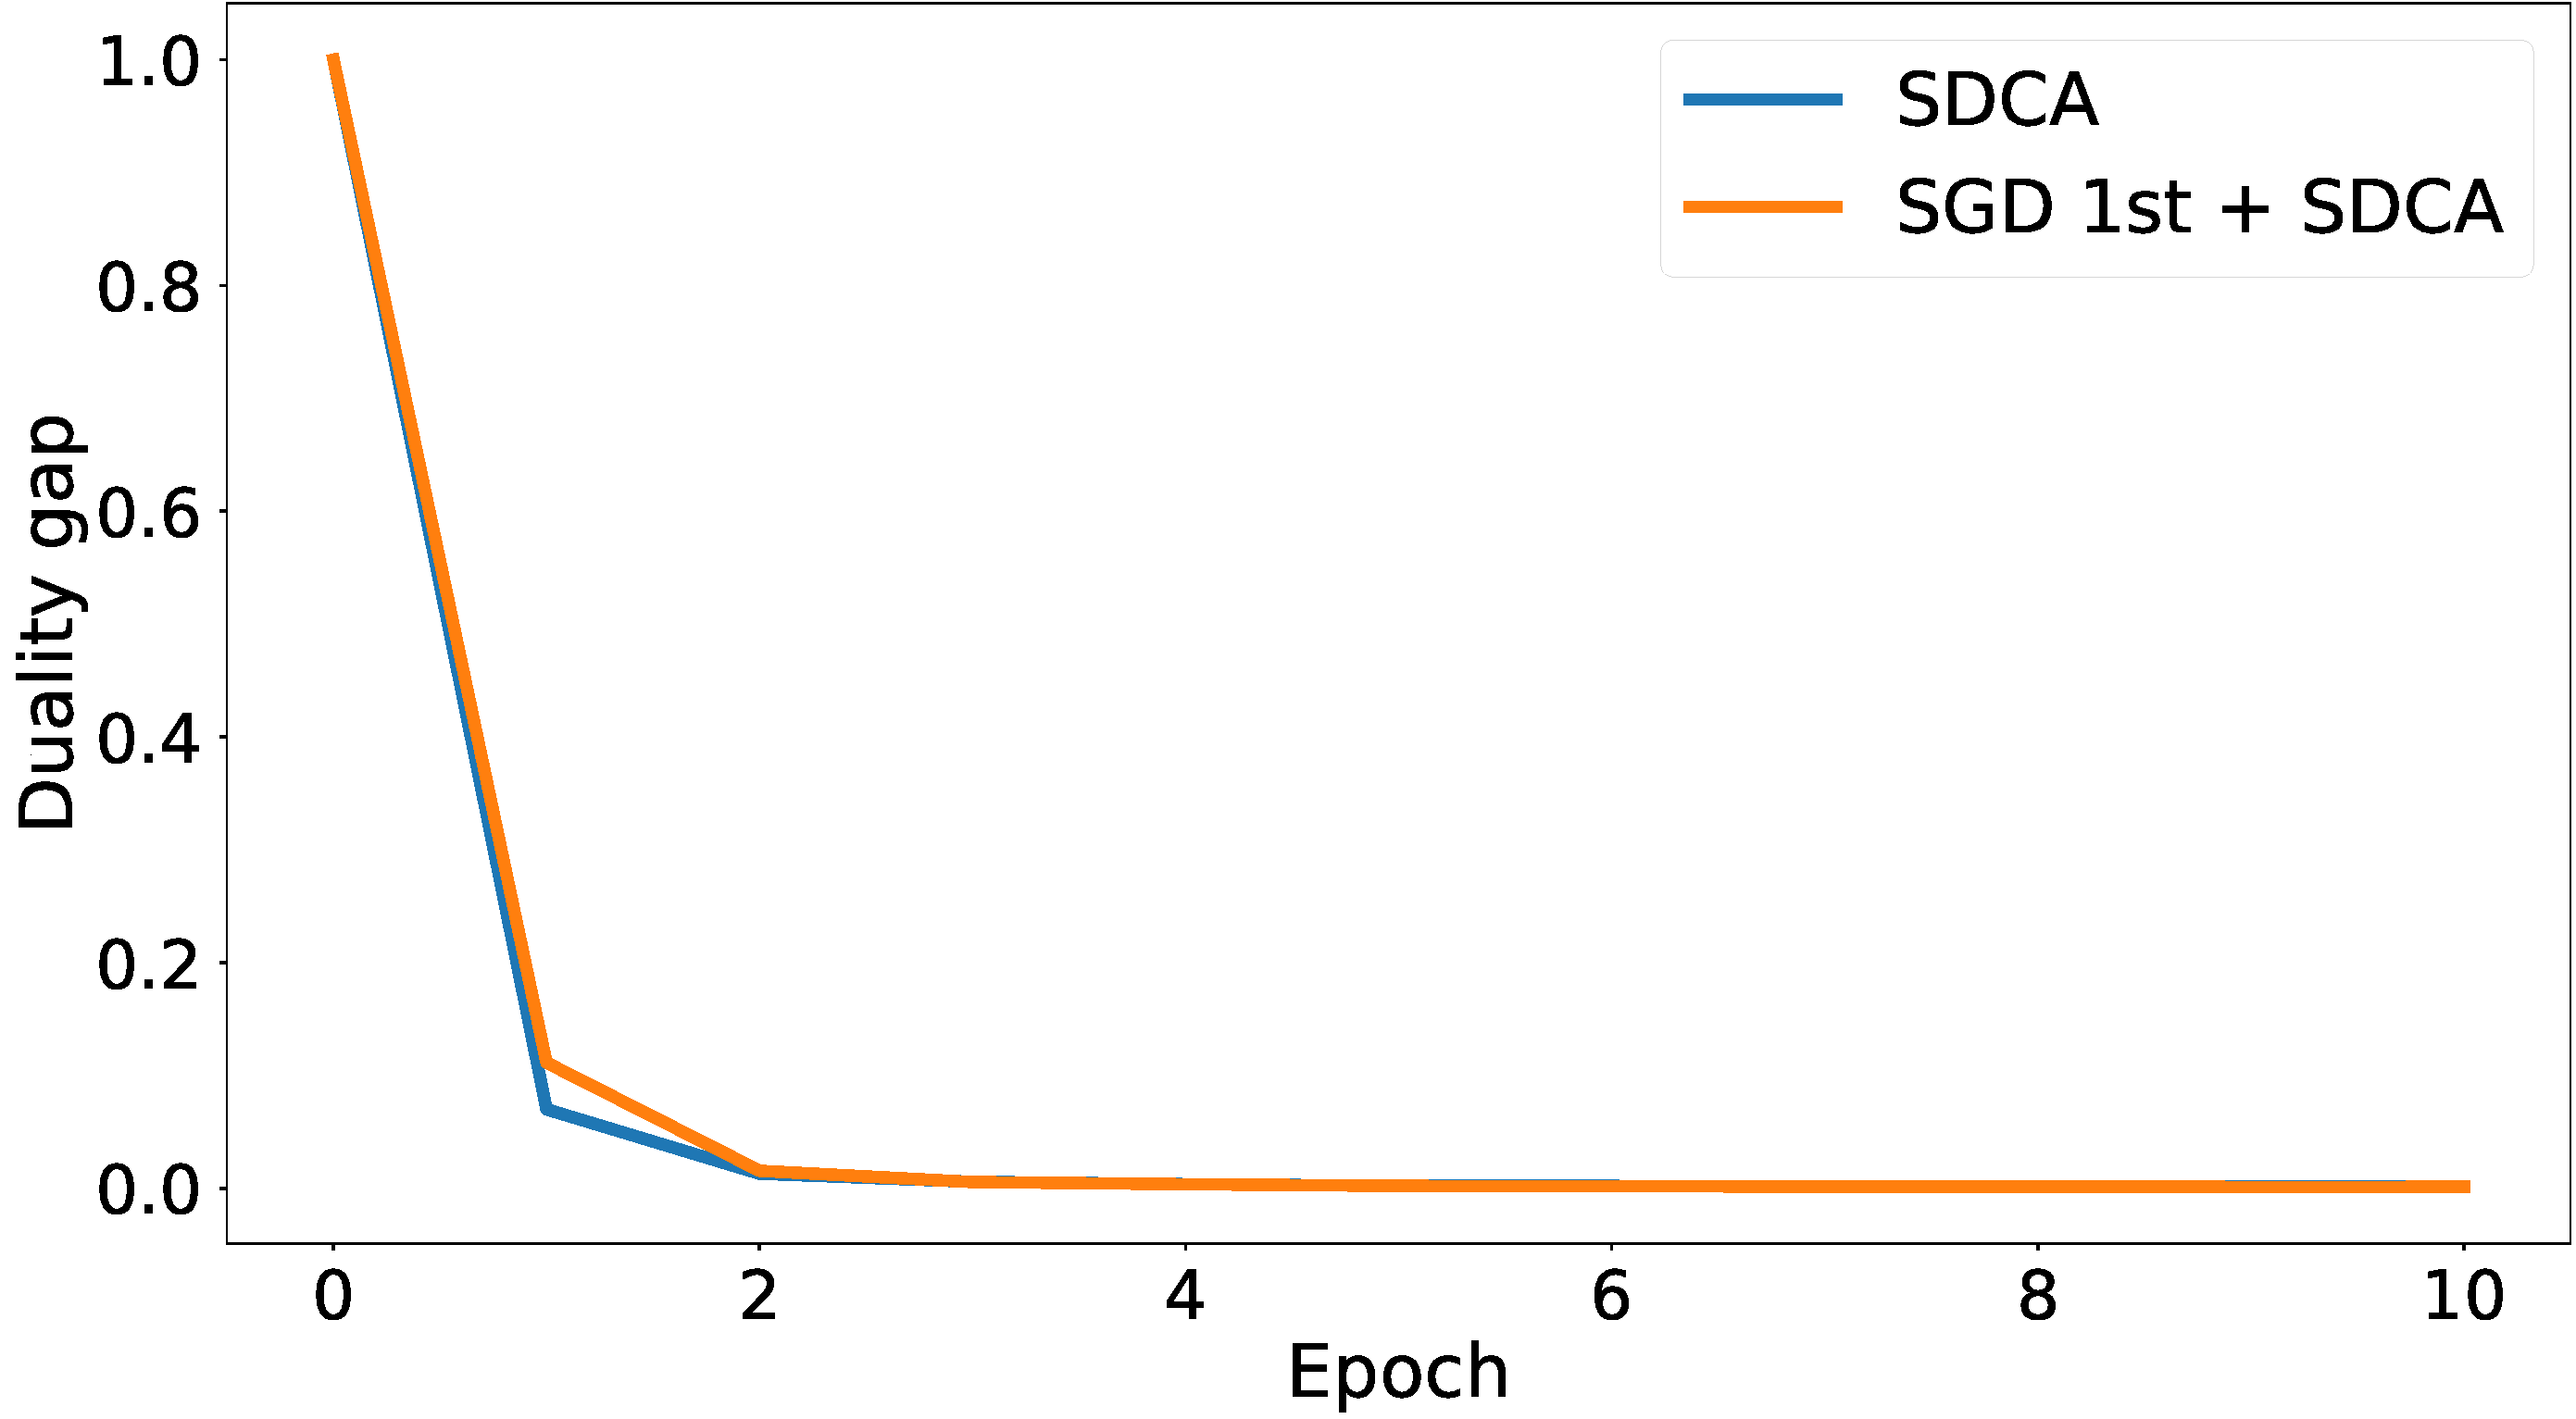
\includegraphics[width=0.55\textwidth]{Graphs/duality_original3_mc100.pdf}
  \caption{Decrease in duality gaps - Cropped vectorized images - averaged over 100 runs - $\lambda = 1.6$}\label{find_centre}
\end{figure}

\FloatBarrier
\section{PCA transformed}

\begin{figure}[!htb]
  \centering
  \subfloat[Cropped neutrophils]{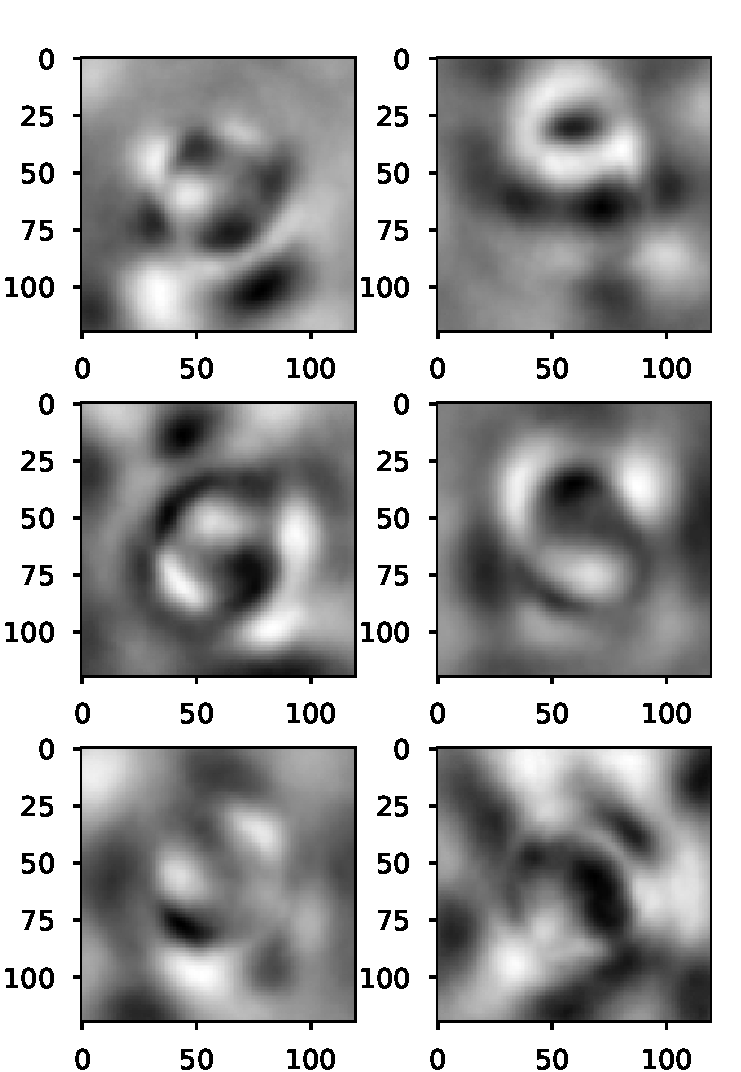
\includegraphics[width=0.36\textwidth]{Graphs/cropped_neutro_pca40.pdf}}
  \hfill
  \subfloat[Cropped lymphocytes]{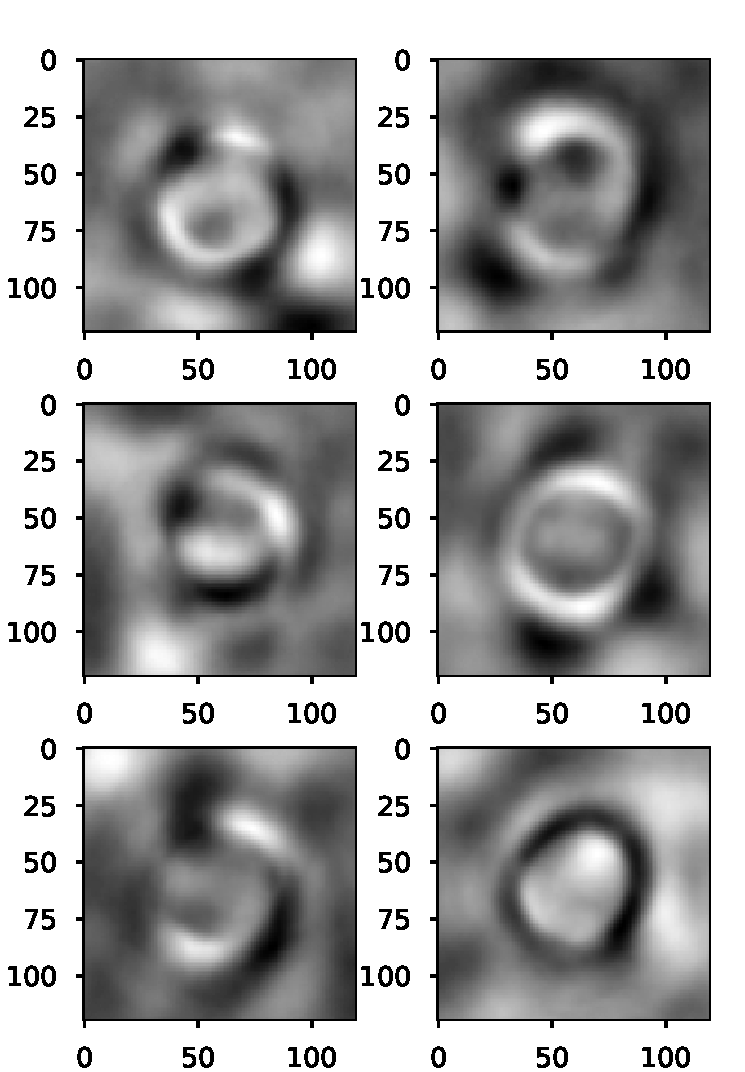
\includegraphics[width=0.36\textwidth]{Graphs/cropped_lymph_pca40.pdf}}
  \caption{PCA transformed images for both classes}\label{pca_reduced}
\end{figure}


\begin{figure}[!htb]
  \centering
  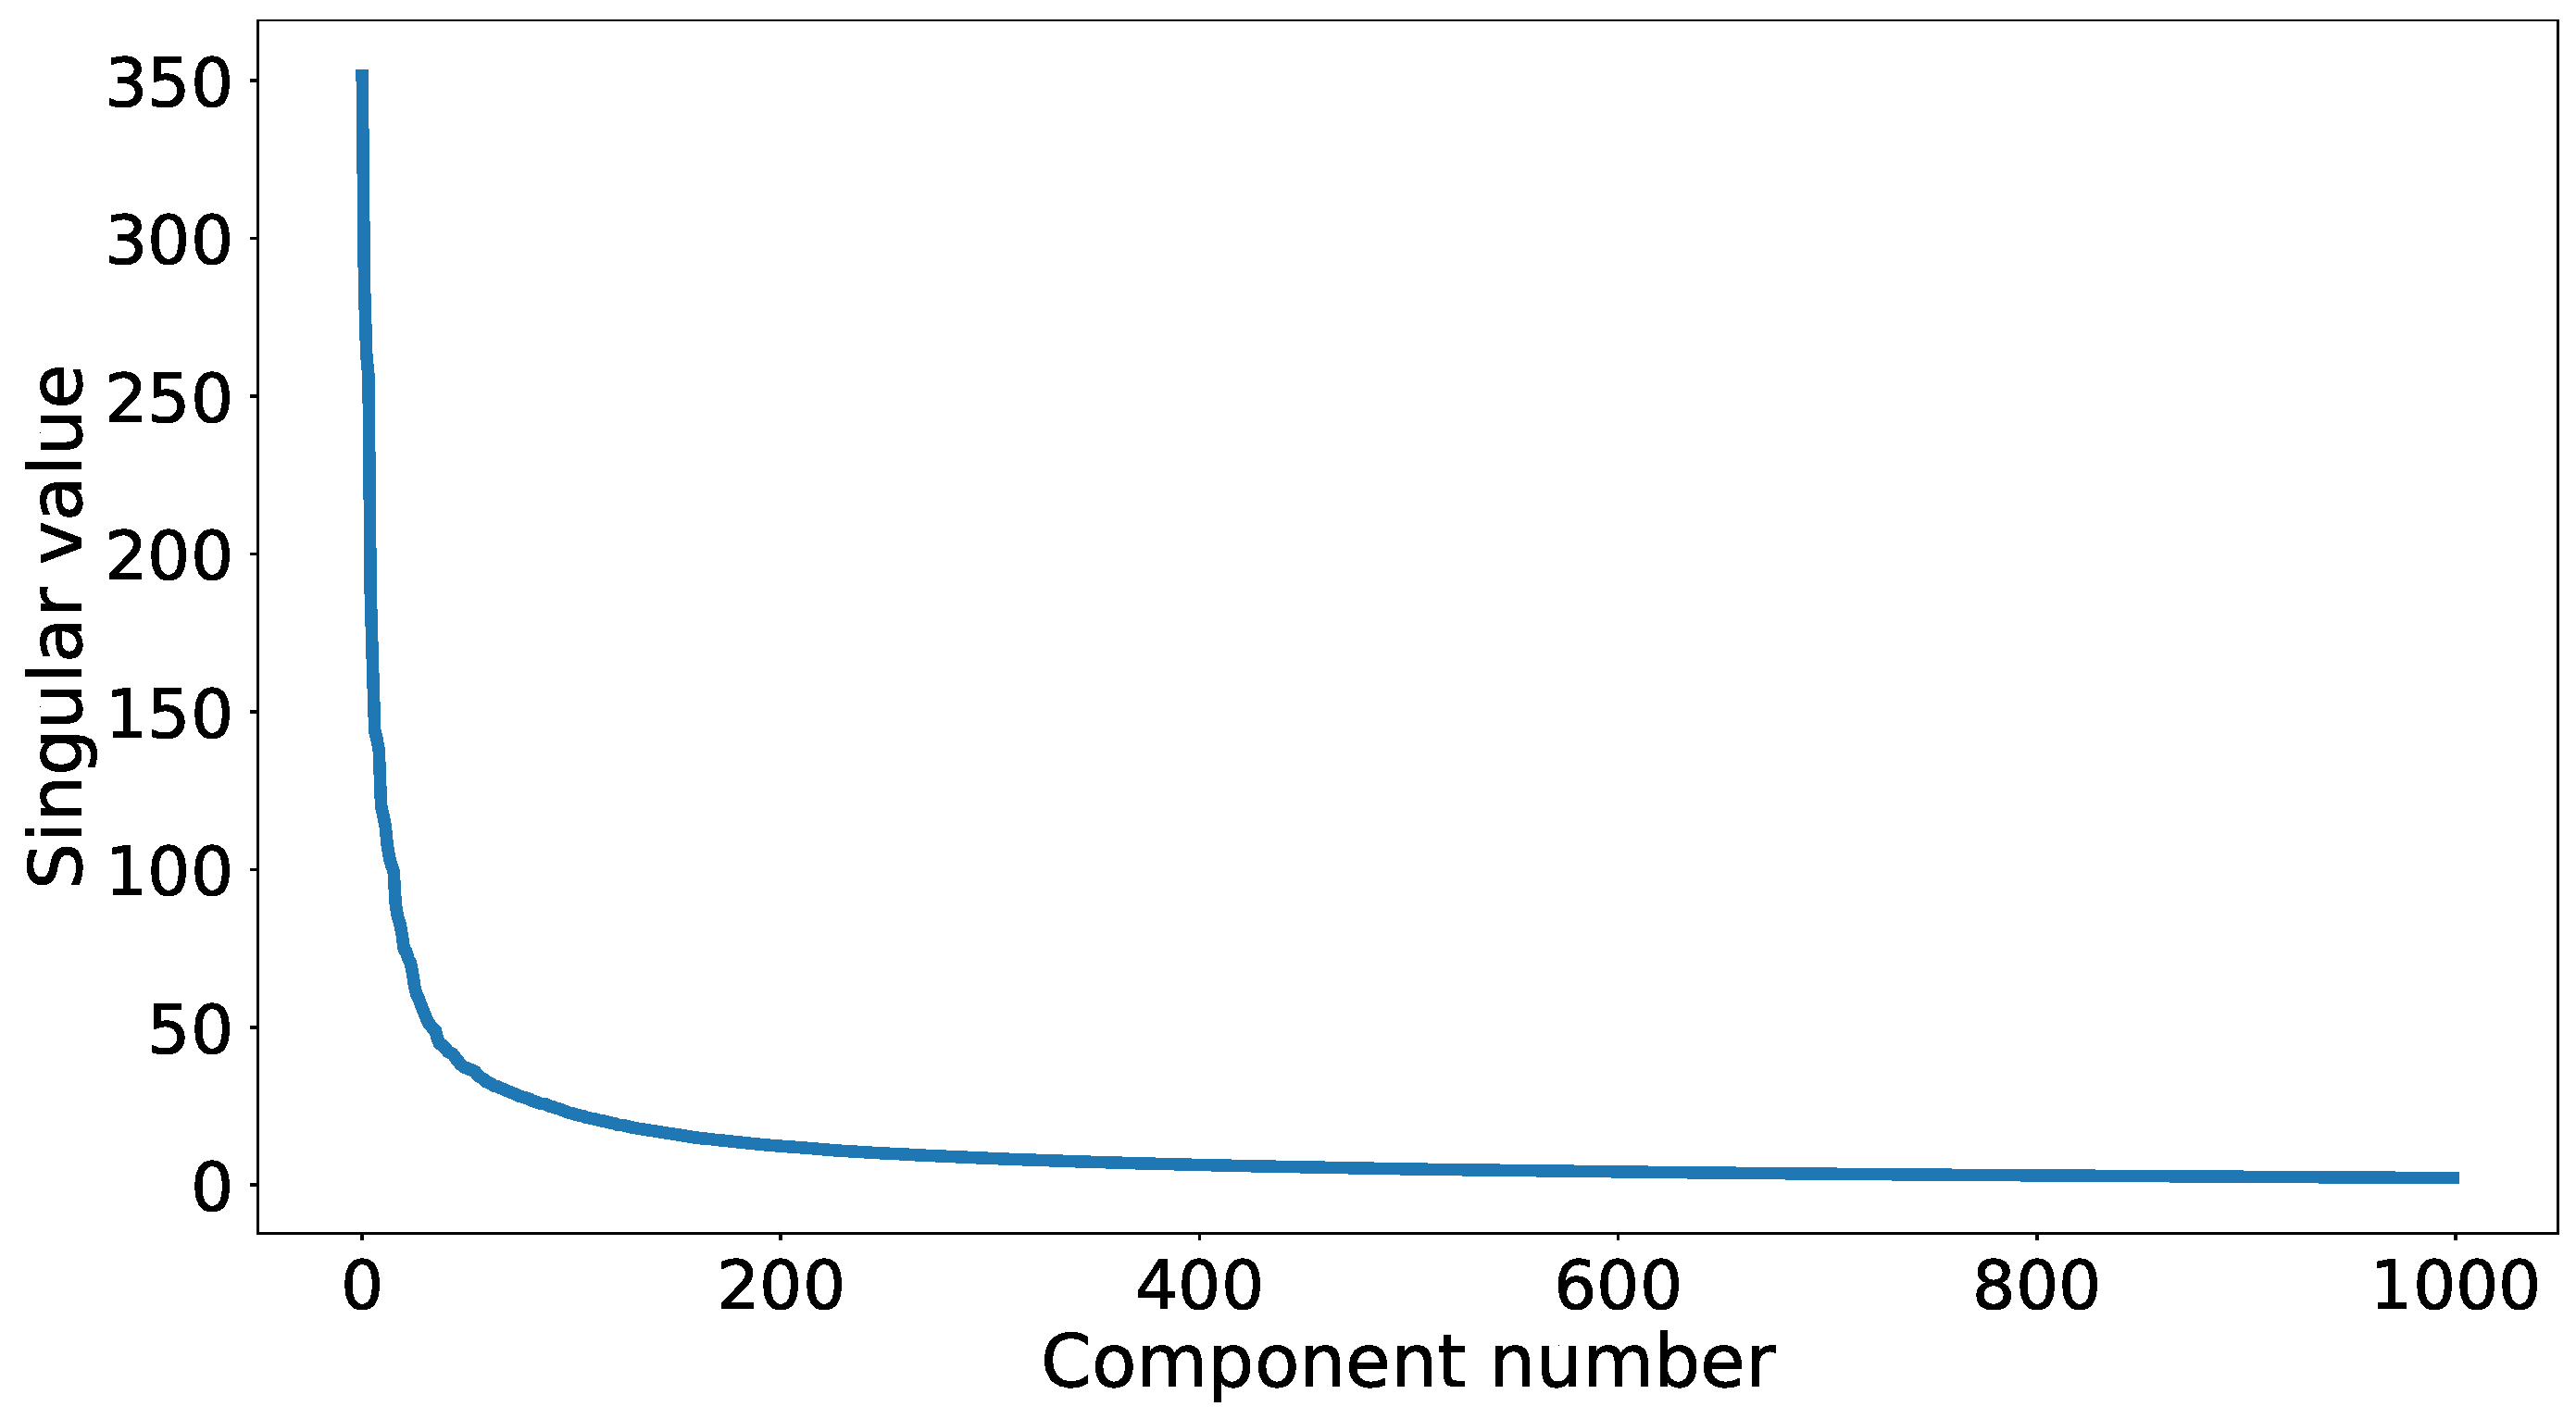
\includegraphics[width=0.55\textwidth]{Graphs/pca_decrease.pdf}
  \caption{Singular values decrease}\label{pca_decrease}
\end{figure}


\end{document}